\documentclass{article}

\usepackage{amsmath}
\usepackage{amsfonts}
\usepackage[left=3cm,right=3cm,top=2.5cm,bottom=2.5cm]{geometry}
\usepackage[sort&compress]{natbib}
\bibliographystyle{apalike}
\usepackage{soul}
\usepackage{url}
\usepackage{circuitikz}
\usepackage{amsthm}
\usepackage{hyperref}
\usepackage{titlesec}
\usepackage{tikz}
\usepackage{caption}
\usepackage{cleveref}

\usetikzlibrary{arrows, positioning, arrows.meta}


\newcommand{\xd}{x_{dist}}
\newcommand{\yt}{y_{temp}}
\newcommand{\indep}{\perp \!\!\! \perp}
\newcommand{\refp}[1]{(\ref{#1})}
\newcommand{\degrees}{$^{\circ}$}
\newcommand{\R}{\mathbb{R}}
\newcommand*\circled[1]{\tikz[baseline=(char.base)]{
            \node[shape=circle,draw,inner sep=2pt] (char) {#1};}}

\newtheorem{theorem}{Theorem}
\newtheorem{definition}{Definition}
\newtheorem{corollary}{Corollary}

\title{Active Inference}
\author{Jack Montgomery}
\date{July 2024}

\begin{document}

\begin{titlepage}
    \centering
    \vspace*{1in}
    
    {\LARGE \textbf{All Things Active Inference}}\\[2cm]
    
    {\large \textbf{Jack Montgomery}}\\[0.5cm]
    {\large MNTJAC003}\\[0.5cm]
    {\large Supervisor: Prof. Jonathan Shock}\\
    {\large University of Cape Town}\\[2cm]
    
    
\includegraphics[width=0.3\textwidth]{images/UCT_logo_circular_blue_large.png}\\[2cm]
    
    {\large September 26, 2024}\\[3cm]
    
    % Abstract section
    \begin{abstract}
INSERT ABSTRACT
    \end{abstract}
    
\end{titlepage}

\newpage

\tableofcontents

\newpage

\section{Introduction}

Active inference is a normative framework that characterises adaptive behaviour through the general paradigm of surprise minimisation. The foundation of this framework is the Free Energy Principle (FEP) \citep{friston2006free}, which is proposed as a unifying theory of cognition \citep{friston2010free}. Active inference can similarly be derived from the assumption of the persistence of biological systems \citep{friston2012active}. Beyond its theoretical grounding, the framework has found applications in diverse fields, such as signal processing in hearing aids \citep{podusenko2022aida} and machine learning \citep{millidge2021applications}. The salient point in introducing these wide-ranging derivations and applications is to emphasise that no single perspective - be it biological, computational, or cognitive - can fully encompass the framework.

\

The difficulty, therefore, for any introduction to the framework is how to do justice to these many perspectives. We have already stated that active inference seeks to characterise adaptive behaviour as surprise minimisation, a description that may seem unusual compared to more conventional definitions. Typically, active inference is defined as the selective sampling of sensory observations in order to minimise \textit{free energy}. Ultimately, these two definitions are equivalent, but the former is chosen in this report to ground the discussion in more familiar language. Although the physiological experience of ``surprise'' does not exactly match its statistical or physical meaning, it helps provide an intuitive understanding of how this framework ties together diverse behaviours under a unified principle. The challenge we face, then, is: how can we characterise both simple biological systems, like cells, and complex systems, like the human brain, as engaging in the same underlying processes? This is the ultimately what the first part of this report aims to motivate through what \citet{parr2022ActiveInference} call the ``low road'' and ``high road'' to active inference. 

\

Along the high road,''we take the minimal assumption that a biological system persists through time. Even with this simple premise, we are committed to some fundamental concepts, such as the idea that the system is distinct from its environment. This distinction is formalized by the notion of a Markov blanket—a boundary that separates the system's internal states from external states. Equipped with a Markov blanket, a system implicitly creates a probabilistic representation of its environment (referred to as external states). However, a system cannot simply replicate the dynamics of its environment without eventually dissipating into it. This is where the system’s ``resistance''to the second law of thermodynamics comes into play: a system must actively maintain its integrity to avoid entropy and disorder. We can formalize this resistance by modeling the sensory observations and the biological system as a random dynamical system. Through this lens, we will derive what it means for a system to be ``active''or persist over time, thereby motivating the system's engagement in active inference.

\

Complementary to the high road, we will explore the ``low road''to active inference. This path begins by understanding the brain as a predictive machine, grounded in Helmholtz's theory of perception as ``unconscious inference''\citep{helmholtz1867concerning} and its modern interpretation in the Bayesian brain hypothesis \citep{doya2007bayesian}. We will consider how these theories extend beyond perception to include the sensorimotor system, showing how prediction and inference operate in action. Additionally, we will explore how the integration of bottom-up sensory input and top-down cognitive processes in perception ties into recent studies of neural activity, particularly in visual processing. These theories introduce us to the notion of a generative model of the environment. This generative model allows the brain to perform inference which again will allow us to motivate the brain engaging in active inference.

\

The ideas surrounding active inference that we have discussed so far are not immediately useful from an empirical perspective. The hypotheses themselves are not, by their nature, \textit{falsifiable}. However, how active inference and the Free Energy Principle may manifest in organisms or the brain is a more testable proposition. In this report, we will present two prominent \textit{process theories} that have been developed to explore this manifestation. The first of these is \textit{predictive coding}.

\

Predictive coding is a theory of cortical function that proposes the brain is composed of a hierarchy of neural activity, wherein higher levels predict the activity of the lower levels. The brain’s main objective, according to this theory, is to minimise prediction errors between the levels. This objective is consistent with the minimisation of surprise and, by extension, with active inference. However, classical predictive coding models often deal with static sensory stimuli, which are assumed to be independent. In contrast, real-world sensory inputs are highly correlated over time. This limitation is addressed by a more recent extension of the theory known as \textit{temporal predictive coding}. Fundamentally, temporal predictive coding incorporates the dimension of time into the model, enabling it to deal with the problem of correlated stimuli.

\

Temporal predictive coding provides us with a formal algorithm for perception and learning within our agent. However, planning—a crucial component of active inference—is not included in this model. To address this, we will extend the temporal predictive coding model by incorporating corollaries and components from the active inference framework.

\

Our agent and model will be built by considering different cortical functions such as perception, learning, and planning. For each of these, we will define analogous algorithms within our model that connect the statistical inference to cognitive functions. To demonstrate these ideas, we will develop an agent within the \textit{adaptive Bayesian thermostat} environment. This environment, introduced by \citet{buckley2017free}, involves a simple task: the agent must infer its distance from a heat source based on noisy temperature readings. The agent is equipped with a preferred temperature, which it incorporates into its planning to decide on its actions.

\

The adaptive Bayesian thermostat is a simple environment designed to demonstrate the core components of predictive coding and active inference. In addition, we will test the temporal predictive coding model in the CartPole environment from the \textit{OpenAI Gymnasium} package \citep{towers2024gymnasium}. This environment, a classic control problem in the reinforcement learning literature, involves balancing a pole on a cart. Several modifications were made to the environment, including shifting it from a Markov Decision Process (MDP) to a Partially Observable MDP (POMDP), and defining a preference distribution over the agent's observations. We present the results of the model’s performance in this task, along with a discussion.

\

Additionally, we will demonstrate how active inference theories manifest in \textit{message passing} on a factor graph. Message passing has deep roots in theories of cortical computation \citep{parr2019neuronal}, and it is also foundational to many efficient Bayesian inference algorithms. One such algorithm we will implement is \textit{belief propagation}. This model will be tested in another reinforcement learning baseline, the Mountain Car environment.

\

By applying this framework to control problems and providing a formal introduction to the underlying theories, we aim to offer the reader both a clear understanding of the rich normative theory behind active inference and an appreciation for its wide-ranging practical applications.

\section{Review of Related Work}

The foundations of active inference lie in the Free Energy Principle \citep{friston2006free}. In this seminal work, Friston combines the Helmholtzian idea of perception with the concept of free energy minimisation from statistical physics to formulate a principle applicable to the brain. He argues that the problems of inferring the causes of sensory input and learning the causal structure of their generation can be resolved through free energy minimisation. In this context, free energy measures the difference between the probability distribution of environmental states affecting the system and the internal model encoded by the system's configuration. A system can minimise free energy in two ways: by altering its internal model, which corresponds to perception, or by changing its interaction with the environment, which corresponds to action. This framework assumes that the system encodes an implicit and probabilistic model of its environment.

\

The Free Energy Principle was further developed in the context of biological systems by \citet{friston2012free}, who approached the environment from the perspective of dynamical systems theory. This separates the system into internal and external states, with only external states susceptible to random fluctuations. The objective is to find the dynamics of internal states that ensure the system remains within a limited set of external states, reducing uncertainty. The proposed solution is motivated by the Hamiltonian Principle of least action, linking the minimisation of free energy to the broader framework of action in physical systems. \citet{millidge2019combining} offers a more accessible introduction to the Free Energy Principle, framing its applications to biological systems in more colloquial language. In contrast to the formalism of \citet{friston2012active}, \citet{millidge2019combining} simplifies the key concepts, making them more intuitive while maintaining their core theoretical integrity. This review aims to balance the formal and intuitive descriptions of active inference, reflecting both perspectives.

\

The works cited above present active inference as a framework for adaptive biological behaviour, grounded in the Free Energy Principle. However, there are multiple ways to approach this framework. \citet{parr2022ActiveInference} introduces the metaphor of the ``high road'' and ``low road'' to active inference. The ``high road'' starts with minimal assumptions — essentially just the persistence of the system — and derives active inference using the Markov blanket and the principle of least action. Which is similar to the perspectives on active inference we have discusses so far. This approach reflects a top-down view, building from general principles toward specific computational mechanisms.

\

On the other hand, the ``low road'' starts with the concept of the Bayesian brain and extends the Helmholtzian idea of perception as unconscious inference to planning as inference. Both forms of inference minimise the same objective: variational free energy. \citet{parr2022ActiveInference} Which promotes the idea that we can adjust our beliefs to better reflect the world as well as, adjust the world to better reflect our beliefs. Using this dual-road metaphor to emphasise that there are many starting points for discussing active inference, reflecting the diversity of approaches in the literature.

\

The second half of \citet{parr2022ActiveInference} explores the practical applications of active inference, detailing specific generative models and process theories associated with the framework. \citet{smith2022} adopts a similarly empirical approach, linking the theoretical underpinnings of active inference to practical, implementable algorithms. \citet{dacosta2020active} focuses on discrete state-space models and provides a ground-up approach to the application of active inference, bridging the gap between theory and practical implementation. This work highlights how active inference is not just a theoretical construct but also a viable framework for modelling intelligent agents in real-world scenarios.

\

When discussing specific implementations, \citet{parr2019neuronal} compares different message passing algorithms, which are proposed as neural process theories underlying active inference. Notably, marginal message passing is contrasted with variational message passing \citep{winn2005variational} and belief propagation \citep{pearl1986prop}. Despite their differences, all these algorithms can be understood as minimsating free energy, albeit with different assumptions about the factorisation of the generative model—such as the mean-field approximation in variational message passing and the Bethe approximation in belief propagation.

\

The majority of the literature on active inference focuses on discrete-state models. However, continuous-state models have also been developed. For instance, \citet{van2019simulating} present an online active inference agent using variational message passing in the mountain car environment, a classic reinforcement learning task. This agent is implemented using a Forney-style factor graph and computes the posterior distribution of its generative model over a defined inference horizon.

\

Message passing, though closely related to active inference, is distinct in that it represents a hypothesis about the physical implementation of active inference in the brain. As such, it is falsifiable, making it a candidate for empirical testing. Another prominent implementation of active inference is predictive coding, where neural circuits minimise prediction errors between hierarchical levels of representation. The foundational work on predictive coding was done by \citet{rao1999predictive}, who modelled visual processing as a hierarchy where higher levels predict lower-level activity and adjust based on the prediction errors.
\

\citet{friston2005theory} extended this work, showing that predictive coding can be understood as approximate Bayesian inference and that synaptic plasticity can be modelled as Hebbian learning, allowing the system to adapt to environmental noise and recognise patterns. Predictive coding has also been extended to handle temporal sequences of stimuli, as detailed by \citet{friston2010filtering}, who introduced the concept of generalised filtering for non-linear state-space models.

\

However, the implementation of predictive coding for dynamic stimuli, particularly with generalised coordinates, poses challenges for neural modelling. In response, \citet{millidge2024temporal} introduced a simpler model called temporal predictive coding, which handles temporal sequences with local connectivity and Hebbian plasticity rules. This approach offers a more biologically plausible alternative to Kalman filtering and addresses the issue of hard-coding temporal dependencies.

\

Finally, \citet{millidge2019combining} combined predictive coding with active inference, allowing agents not only to perceive but also to act in ways that minimise free energy. This hybrid model uses a hierarchical predictive coding network to drive action selection, framing the agent's interaction with the environment as a Partially Observable Markov Decision Process (POMDP). Here, action becomes another variable in the free energy minimisation process, with the agent selecting actions that reduce the divergence between predicted and actual outcomes. This allows the agent to plan and act in a manner that aligns its future states with its goals, providing a practical application of active inference to decision-making.

\section{Theory and Background}

The background and theory section of this paper is inspired by the structure presented in \citet{parr2022ActiveInference}. The goal for this section is to show that from two completely different sets of assumptions or starting points, we are able to derive models and frameworks that represent active inference in their respective contexts.

\

To do this, we will ground ourselves in a definition of active inference that aims to be agnostic to any specific approach, and can be understood intuitively, almost independent of context. The definition we will use is:

\begin{definition}[Active Inference]

Adaptive systems will change their beliefs about the outside world, as well as change the outside world itself, to reduce the surprise of their observations.

\end{definition}

Crucially, this definition hinges on the notion of ``surprise''. While the meaning of surprise may vary across domains (as we will see in random dynamical systems versus statistical contexts), the central premise remains consistent. This foundation enables us to demonstrate the broad applicability of active inference across different frameworks and interpretations.


\subsection{High Road to Active Inference}

If a biological organism is surviving in an environment governed by the second law of thermodynamics, what must it \textbf{necessarily} be doing?

\

Biological systems, and in particular living organisms, are typically fragile in terms of the range of states they can occupy. For instance, the human body functions within a narrow temperature range - normally around $37^\circ$ - with fevers pushing this to around $40^\circ$, a relatively tight margin for survival. Additionally, living systems are constantly exposed to random fluctuations from their environment, which, due to the second law of thermodynamics, tend to push their internal states towards disorder, often beyond their viable limits \citep{friston2012free}. Given this inherent fragility and the random nature of environmental influences, the critical question becomes: how do biological systems adapt to resist these fluctuations and maintain their state within their viable bounds?

\

Before diving further into this question, it is essential to establish the distinction between the system and its environment. The persistence of any system over time implies a boundary between itself and the external world—a boundary that can be formalised as a \textit{Markov blanket}.

\subsubsection{Markov Blankets}

It is essential that any adaptive system maintains both structural autonomy and separation from its environment. Without this, the system would merely dissolve into the environment's dynamics \citep{parr2022ActiveInference}. This separation is statistically formalised by the existence of a Markov blanket \citep{pearl1988Probabilistic} between a system and its environment:

\begin{definition}[Markov Blanket]\label{def:markov_blanket}
A Markov blanket, $b$, is defined as:
$$ \mu \indep x \  | \ b \iff p(\mu, x | b) = p(\mu | b) p(x | b) $$
\end{definition}

This means that when a blanket $b$ is present, the variable $x$ is independent of $\mu$ given $b$. Said another way, this defines a conditional independence between the random variables $x$ and $\mu$.

\

A Markov blanket is a set of variables that mediate the interaction between a system and its environment. A specific example of a dynamic Markov blanket is illustrated in Figure \ref{fig:markov_blanket}, where external states of the environment are statistically separated from the internal states of the adaptive system. Additionally, two intermediary states - sensory and action states, known as the \textit{blanket states} - are identified. 

\

Thus, by assuming the existence of this Markov blanket, we assert that knowing the active and sensory states provides no further information about the external states when it comes to the internal states. This is typically interpreted as the idea that internal states cannot \textbf{directly} influence external states; instead, they affect them \textbf{indirectly} via the active states. Similarly, external states cannot directly alter internal states but can only affect them through sensory states.


\begin{figure}[htbp]
    \centering
    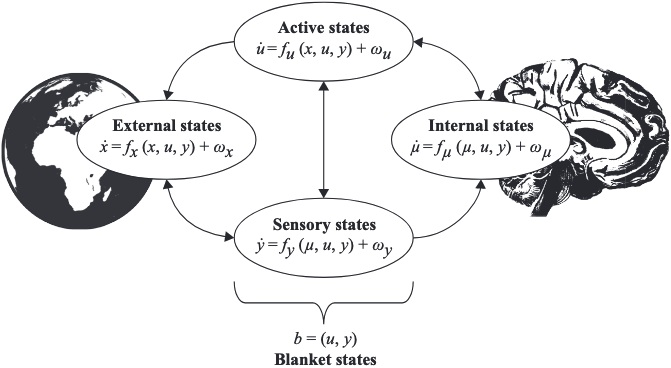
\includegraphics[scale=0.55]{images/markov_blanket.png}
    \caption{Example of a dynamic Markov blanket from \citet{parr2022ActiveInference} which separates an adaptive system, which in this case is a brain, with its environment. The dynamics of each set of states is determined by a deterministic flow specified as a function, $f$. This gives rise to the average rate of change and additional random fluctuations, $\omega$. With arrows indicating the direction of influence between the states.}
    \label{fig:markov_blanket}
\end{figure}

\

The key point is that internal and external states are formally related across the Markov blanket, as both influence and are influenced by the blanket states. Because of this, we can construct conditional probability distributions for the internal and external states, given the blanket states. These distributions are conditioned on the same blanket states, allowing us to associate pairs of expected internal and external states with each other. In other words, on average, internal and external states achieve a form of synchrony. This implies that if we can define independent distributions over external and internal states given their Markov blanket, the two states become informative about each other through the blanket. This synchrony gives internal states the appearance of representing or modelling external states.

\

\begin{figure}[htbp]
    \centering
    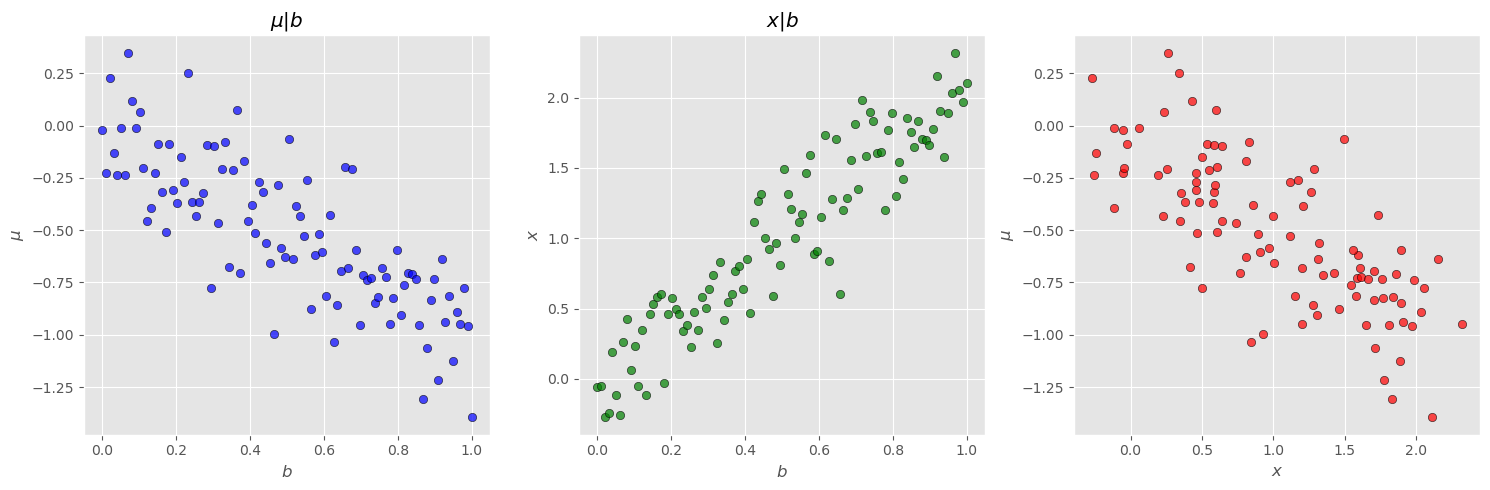
\includegraphics[scale=0.4]{images/blanket_prob_relation.png}
    \caption{Example of how two random variables $x$ and $\mu$, both conditioned on the blanket state $b$ can impose some probabilistic representation of the other. \textbf{Left}: Depicts the data generated from $\mu|b$. \textbf{Middle}: Shows the data generated from $x|b$. \textbf{Right}: Depicts how these variables have a synchrony based on being conditioned on the same blanket states. The line depicted is the result of linear regression on $\mu$ using variable $x$.}
    \label{fig:markov_blanket_prob_relation}
\end{figure}


From a Bayesian perspective, the dynamics of the internal states correspond to a form of approximate Bayesian inference about external states \citep{parr2022ActiveInference}. Since as sensory states change, the associated internal representation is updated through an implicit model of how sensory states are generated. However, the agent’s model cannot simply mimic external dynamics, as this would cause the agent to dissolve into the external environment — similar to why we introduced the concept of a Markov blanket. Instead, the model must encode a preference for certain sensory states. These preferences can be specified in terms of more likely states in the model’s prior distribution. Under this formulation, optimal behaviour — relative to the agent's prior preferences — can be viewed as the maximisation of model evidence through perception and action \citep{parr2022ActiveInference}. This suggests that the system engages in \textit{self-evidencing} \citep{hohwy2016evidencing}, meaning the system acts to acquire sensory states that align with its internal model, thereby maximising model evidence. We will return to these ideas later in this section. 


\subsubsection{Random dynamical system}

While noting that this Markov blanket is indeed necessary for a biological system's persistence over time - the question that we posed initially is what must a system be \textbf{doing} to ensure its persistence over time. Our hypothesis for this was the system was required to keep certain internal parameters within small viable bounds. We can formalise this by describing the system and the sensory states as a random dynamical system. 

\

A random dynamical system consists of two components: a \textit{base flow} and a \textit{dynamical system} on some physical space $X \in \R^d$.

\

The base flow, $\vartheta: \Omega \to \Omega$, is comprises measure-preserving measurable functions: $\vartheta_t: \Omega \to \Omega$ for each time $t \in \R$. These functions form a group of transformation of a probability space $(\Omega, \beta, P)$, such that $(\Omega, \beta, P, \vartheta)$ is a measure preserving dynamical system with $\sigma$-algebra $\beta$ defined on $\Omega$ and $P: \beta \to [0, 1]$ is a probability measure.

\

The dynamical system $(R^d, \varphi)$ comprises of a solution operator: $\varphi: \R \times \Omega \times X \to X$. Which is a measurable function that maps to the metric state space $X \subseteq \mathbb{R}^d$. This function satisfies the \textit{cocycle} property: $\varphi(\tau, \vartheta_t(\omega)) \circ \varphi(t, \omega) = \varphi(t + \tau, \omega)$. This solution operator can be considered as the solution $x(t) = \varphi(t, \omega)(x_0)$ to a stochastic differential equation of the form:

\begin{equation}
	\begin{aligned}
		\dot{x}(t) &= f_X(x) + g_X(x)\omega(t) \\
		x(0) &= x_0
	\end{aligned}
\end{equation}

In all following derivations, we denote random dynamical systems as a tuple: $m = (\R^d, \varphi)$.

\

Crucially, we allow for a partition of the state space $X = R \times S$ , where $R \subset X$ is distinguished by  the existence of a map $\varphi_R : R \times X \to R$ that precludes direct dependency on the base flow. In this  sense, $R$ constitutes an internal state space, while $S \subset X$ constitutes an external state space. Which we allow to give rise to the external mapping: $\varphi_S: \R \times \Omega \times A \times S \to S$. That may only depend on a subset of internal states $A \subset R$. 

\

In this set up, internal states have dynamics that depend on external states and themselves, while external states depend on internal states and themselves but are also subject to fluctuations. See Figure \ref{fig:random_dynamical_system} for a representation of these dynamics.

\begin{figure}[htbp]
    \centering
    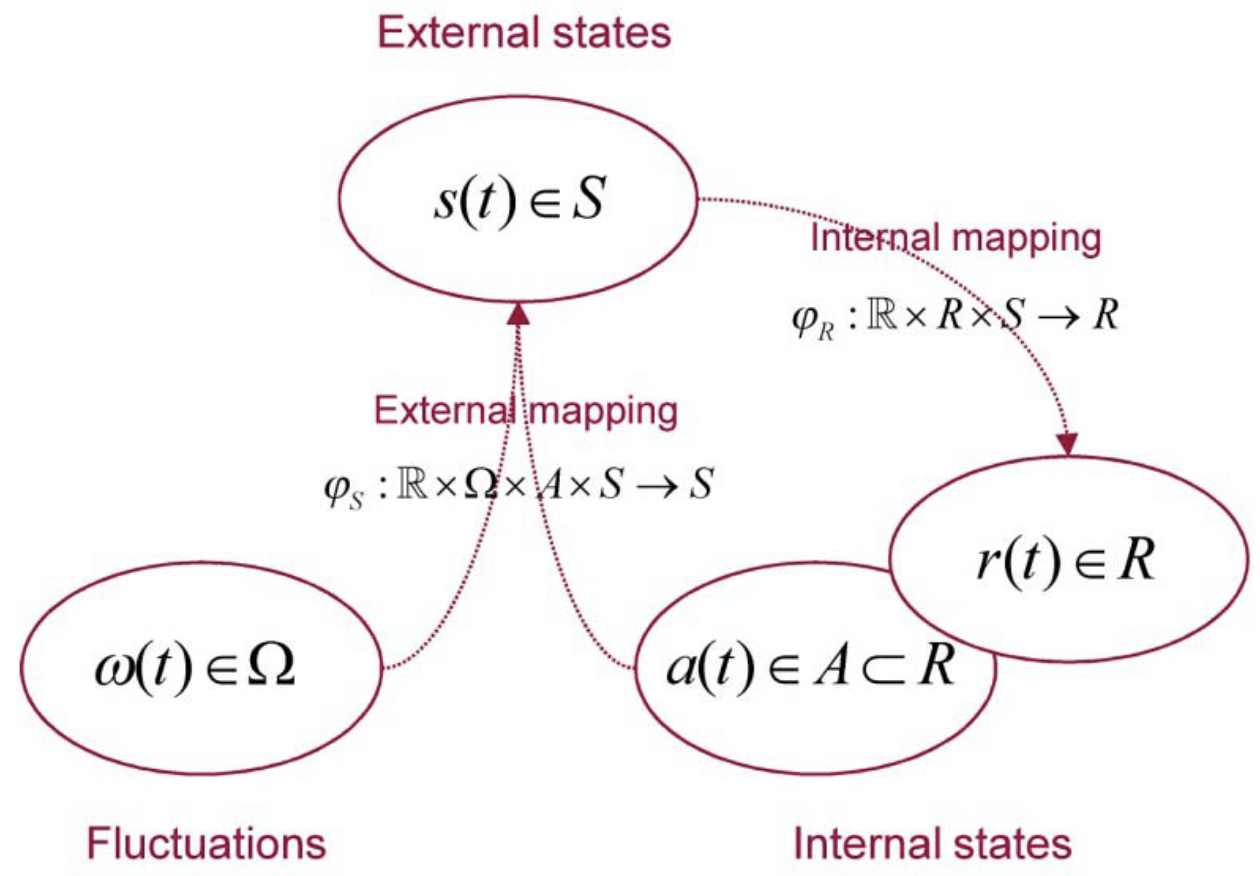
\includegraphics[scale=0.5]{images/random_dynamical_system.png}
    \caption{Image from \citet{friston2012free} depicting the component of described random dynamical system. The nodes denote spaces and subsets, while lines depicts mappings with their arrows denoting the direction of influence.}
    \label{fig:random_dynamical_system}
\end{figure}

\paragraph{Remark} The use of external states and internal states here is done to be consistent with \citet{friston2012active}. There may be some confusion, as ``external states'' described in this dynamical system can be more closely associated with ``sensory states'' in the Markov Blanket (Figure \ref{fig:markov_blanket}).

\

We are interested in biological systems in this discussion thus we can regard the external states $s(t) = \varphi_S(t, \omega)(x_0)$ as the state of the sensory receptors, while the internal states $r(t) = \varphi_R(t)(x_0)$ that include $a(t) \in A \subset R$, respond to sensory perturbation. We will refer to $a(t)$ as active states since they control how environmental fluctuations are sampled by sensory states.

\subsubsection{Active states and principle of least action}

We aim to study systems whose physical states, $x(t) = \varphi(t, \omega)(x_0)$, are confined to a bounded subset of states and remain there indefinitely. This is what we have defined as necessary for a system's persistence. Within random dynamical systems, this means the system possesses a random dynamical attractor, which we assume is ergodic. This is a compact set $\mathcal{A}(\omega) \subset X$ which. is invariant under the flow map such that  $\varphi(t, \omega)(\mathcal{A}(\omega)) = \mathcal{A}(\vartheta_t(\omega))$. In terms of ergodic theory, this means there is a unique and stationary ergodic density $p(x | m)$ that is proportional to the amount of time each state is occupied. This density can then be characterised by:

\begin{equation}\label{eq:ergodic_density}
	p(s | m ) = \lim_{T \to \infty} \frac{1}{T} \int^T_0 \delta( x - x(t)) \ dt \ a.s
\end{equation}

The ergodic density $p(x | m)$ is an invariant probability measure that can be understood as the  probability of finding the system in any state when observed at a random point in time. The existence of the ergodic density and its underlying attractor ensures the system has invariant characteristics that underwrite its existence over time. 


\begin{definition}[Active System]\label{def:active_system}
	An ergodic dynamical system $m = (\R^d, \varphi)$ is said to be active if it possesses an internal map that satisfies the (locally) extremal condition:
	\begin{equation*}
	\begin{aligned}
		\varphi_R^*= \text{argmin}_{\varphi_R} H(S | m) \\
		H(S | m) = - \int p(s | m)\ln p(s | m)
	\end{aligned}
	\end{equation*}
\end{definition}

In other words, the internal states of an active system minimise the entropy over the external states. Which means that internal states of an active system minimise the dispersion of their external states. Which gives a formal representation of the hypothesis stated at the beginning of this section. The final link that is needed is between surprise and active systems. This link is found in the Principle of Least Action:

\begin{theorem}[Principle of Least Action]\label{theorem:principle_of_least_action}
The internal states of an active system minimise the Lagrangian or surprise, $\mathcal{L}(s(t))$, such that the variation $\delta_t \mathcal{S}$ of action $\mathcal{S}$ with respect to its internal states vanishes $r(t) \in R$ vanishes.
$$
\begin{aligned}
r(t) & =\varphi_R^*(t)\left(x_0\right)=\arg \min _r \mathcal{L}(s(t)) \iff \partial_r \mathcal{L}(s(t))=0 \iff \delta_r \mathcal{S}=0 \\
\mathcal{S} & =\int_0^T \mathcal{L}(s(t)) \ dt
\end{aligned}
$$
\end{theorem}

\begin{proof}
	We can relate the entropy of the ergodic density $P(s(t) | m)$ in an active system using the ergodic theorem:
	
	$$
	H(S | m) = - \int p(s | m)\ln p(s | m) = - \lim_{T \to \infty} \frac{1}{T} \int_0^T dt \ln p(s(t) | m) = \lim_{T \to \infty} \frac{1}{T} \int_0^T \mathcal{L}(s(t)) \ dt
	$$
	
	This means that for large enough $T$, we can specify:
	
	$$
	T \mathcal{H}(S | m) = \int_0^T \mathcal{L}(s(t)) \ dt = \mathcal{S}
	$$
	
	This equivalence means that $\delta_r\mathcal{S} = 0 \iff \delta_r\mathcal{H}(S | m) = 0 \iff \text{argmin}_{\varphi_R} H(S | m)$. Moreover, $\partial_r \mathcal{L}(s(t)) = 0 \iff \delta_r \mathcal{S} = 0$ by the  fundamental Lemma of variational calculus.
\end{proof}

Since we have assumed that active states, $a(t)$, are a subset of the internal states of the biological system. The Principle of Least Action can be summarised as saying that a biological system minimises the surprise of sensory states by adjusting its internal states, including active states. Which means that a persistent biological system is performing active inference.

\subsubsection{Remark on the relation to Free Energy Principle}

The previous derivations are based on \citet{friston2012active}. Active inference is defined differently in this thesis. It is derived as a Corollary to the \textit{Free Energy Principle}. The derivation of active inference in this regard bears a close relation to (approximate) Bayesian inference and variational free energy derivation of active inference that will be done along the ``low road''. Although, we have completed our goal to show that a persistent biological system must be conducting active inference - we will finish this section true to \citet{friston2012free} and that definition of active inference.

\subsubsection{Free Energy Principle and Active Inference}

The fundamental issue with our current formulation is how internal states can minimise surprise given that they do not know the effect they will have on external states. We have answered \textbf{why} this is required, but we have not discussed \textbf{how} it can be done.

\

Intuitively, the solution regards the system as optimising a probabilistic model of the external dynamics, which is used to minimise surprise. This solution was mentioned in the previous section on Markov blanket when it was remarked that internal states create some implicit model of the external states through the conditioning on the blanket.

\begin{definition}[Generative Model]\label{def:generative_model}
Let $p(s(t)|m)$ be defined as in Definition \ref{def:active_system}, be expressed in terms of some arbitrary parameters $\psi(t) \in \Psi$ that are themselves random variables. We define the generative model as:

\begin{equation*}
	\begin{aligned}
		p(s(t), \psi(t)) &= p(s(t)|\psi(t))p(\psi(t)) \\
		p(s(t)) &= \int_\Psi p(s(t), \psi(t)) \ d\psi
	\end{aligned}
\end{equation*}
\end{definition}

Where $p(s(t))$ is called the marginal likelihood. 

\

Further, we define the proposal distribution, $q$, which plays the role of an arbitrary probability density over the parameters of the generative model. The probability density is parameterised by some subset of the internal states of the system, $\mu(t)$. Crucially, this proposal density is over the variables that parameterise the marginal likelihood of the external states. This allows us to define free energy for a biological system:

\begin{definition}[Proposal Distribution]\label{def:proposal_distribution}
Let $q(\psi(t) | \mu(t))$ denote a mapping $q: R \times \Psi \times R \to R$. This serves as an arbitrary probability density defined over the parameters of the generative model called the proposal density. Further let this density be parameterised by $\mu(t) \in R$ with $\mu(t) \subset r(t)$. 
\end{definition}

A point to note is that $\psi \in \Psi$ are not observable quantities. They are induced with a proposal density and only exist to parametersise the marginal likelihood of external states. This quantities are often referred to as \textit{hidden states}.

\begin{definition}[Free Energy]\label{eq:free_energy}
Free energy is now defined in terms of the proposal and generative  densities as the following expectation:
$$
F(x(t)) = \int_\Psi q(\psi(t) | \mu(t))\ \ln\frac{q(\psi(t) | \mu(t))}{p(s(t), \psi(t))} d\psi
$$
\end{definition}

\begin{theorem}[Free Energy Principle]\label{theorem:free_energy_principle}
Let $ m = (\R^d, \varphi)$ be an ergodic random dynamical system with state space $X = R \times S \in \R^d$. If the internal states $r(t) \in R$ minimise free energy then the system conforms to the principle of least action and is an active system. By the principle of least action \refp{theorem:principle_of_least_action}:

$$
r(t) = \varphi_R^*(t)(x_0) = \text{argmin}_{r} \mathcal{F}(x(t)) \Rightarrow \delta_r \mathcal{S} = 0 \\
$$
\end{theorem}

\begin{proof}
	We can express Free Energy as:
	\begin{equation}\label{eq:free_energy_decomposition}
	\begin{aligned}
		F(x(t)) &= \int_\Psi q(\psi(t) | \mu(t))\ \ln\frac{q(\psi(t) | \mu(t))}{p(s(t), \psi(t))} d\psi \\
		&= \int_\Psi q(\psi(t) | \mu(t))\ \ln\frac{q(\psi(t) | \mu(t))}{p(\psi(t) | s(t), m)} d\psi - \ln p(s(t) | m) \\
		&= \mathcal{L}(s(t)) + D_{KL}\left[ \psi(t) | \mu(t) \| p(\psi(t) | s(t), m) \right]
	\end{aligned}
	\end{equation}
	By Gibbs' inequality, $D_{KL} \geq 0$, therefore free energy is minimised with respect to $\mu(t) \in R$ when the KL-Divergence is 0 (If such a solution exists). This means that $\mathcal{F}(x(t) = \mathcal{L}(s(t))$ and its variation with respect to $a(t) \in R$ vanishes:
	
	$$
	a(t) = \text{argmin}_a\mathcal{F}(x(t)) \Rightarrow \partial_a \mathcal{F}(x(t)) = 0 \Rightarrow \partial_a \mathcal{L}(s(t)) = 0 \Leftrightarrow \delta_a \mathcal{S} = 0
	$$
	
	From \refp{theorem:principle_of_least_action} we see that surprise does not depend on $\mu(t)$, which means $\partial_\mu \mathcal{L}(t) = 0 \Leftrightarrow \delta_\mu \mathcal{S} = 0$ and therefore $\delta_r \mathcal{S} = 0$.
\end{proof}

\paragraph{Remark} In this proof, we have claimed that when minimised the KL-Divergence between the conditional distribution and proposal density is zero. This rests on the assumption that the proposal density can have the same form as the conditional density. This corresponds to \textit{exact} Bayesian inference. When this assumption is relaxed - free energy becomes an upper bound on surprise and the inference is \textbf{approximately} Bayesian. 

\begin{corollary}[Bayesian inference]\label{cor:bayesian_inference}
	Systems that conform to the free energy principle represent the causes of their sensory states in a Bayesian sense: This follows from \refp{eq:free_energy_decomposition}, where minimising free energy with respect to the internal states minimises the divergence between the proposal density and the posterior density over the parameters of the likelihood function:
	
	\begin{align*}
		\mu(t) & =\arg \min _\mu \mathcal{F}(x(t)) \\
		& =\arg \min _\mu D_{K L}(q(\psi(t) | \mu(t)) \| p(\psi(t) | s(t), m))
	\end{align*}
\end{corollary}

In other words, the optimal proposal density $q(\psi(t) | \mu(t))$ - parameterised by internal states becomes the posterior $p(\psi(t) | s(t), m)$, under the model entailed by the system.

\begin{corollary}[Active Inference]
	Systems that conform to the free energy principle will selectively sample what they `expect to see'. This follows from a final rearrangement of free energy in terms of complexity and accuracy or the log likelihood of sensory states under the proposal density:
	
\begin{align*}
	\mathcal{F}(x(t)) & =\int_{\Psi} q(\psi(t) | \mu(t)) \mathcal{L}(s(t)) d \psi+\int_{\Psi} q(\psi(t) | \mu(t)) \ln \frac{q(\psi(t) | \mu(t))}{p(\psi(t) | s(t), m)} d \psi \\
		& =\int_{\Psi} q(\psi(t) | \mu(t)) \ln \frac{q(\psi(t) | \mu(t))}{p(\psi(t) | s(t), m) p(s(t) | m)} d \psi \\
		& =D_{K L}(q(\psi(t) | \mu(t)) \| p(\psi(t) | m))-\int_{\Psi} q(\psi(t) | \mu(t)) \ln p(s(t) | \psi(t), m) d \psi \\
		a(t) & =\arg \min _a \mathcal{F}(x(t)) \\
		& =\arg \max _a \int_{\Psi} q(\psi(t) | \mu(t)) \ln p(s(t) | \psi(t), m) d \psi
\end{align*}

\end{corollary}


This is what \citet{friston2012active} defines as active inference and manifests as a selective sampling of (typical) sensory states that are most likely under the system's posterior beliefs, by Corollary \refp{cor:bayesian_inference}.

\subsection{Low Road to Active Inference}

Humans and other animals live in a world of sensory uncertainty. Through, introspection may tell us that perception is deterministic, many factors contribute to limiting the reliability of sensory information about the world. For example the mapping of 3D objects into a 2D image, neural noise introduced in early stages of sensory coding, and structural constraints on neural representations and computations \citep{knill2004bayesian}. Our brains must effectively deal with the resulting uncertainty to generate perceptual representations of the world and to guide our actions.

\

With aid from advances in artificial intelligent - researchers have begun to rigorously apply concepts of probability theory into perception. \citep{knill2004bayesian} One striking observation from this work is the ways in which human observers behave as Bayesian optimal observers. A correspondence which has fundamental implications for neuroscience, particularly for neural representations of cortical functions like perception and learning. \citep{trommershauser2003statisticalb, trommershauser2003statisticala}

\subsubsection{Hallucinations in perception}

One of the earliest and perhaps most well-known investigations into hallucinations in perception was conducted by Wilder Penfield. \citep{penfield1961activation} Penfield suggested that the cortex is capable of producing percepts based on past experiences, even in the absence of current sensory input. He referred to the temporal lobes as the ``interpretive cortex'', believing that this region was responsible for interpreting the world through past experiences, based on his observations of the temporary hallucinations induced by electrical stimulation on patients. These hallucinations often included hearing familiar voices, musical tunes, or the sight of objects, which seemed to the patients like flashbacks from their past. The subjects' feedback led Penfield to believe that these memories were experienced within a brief episodic context, placed either in the present or the past. Hence, he coined the term interpretive cortex. \citep{knill2004bayesian}

\

Penfield was reluctant to definitively state whether the memories themselves or merely their interpretations were elicited by the electrical stimulation of the temporal cortex. However, the most parsimonious interpretation suggests that memories of sounds, objects, or people are distributed across the cerebral cortex rather than being stored in a specific region. The medial temporal lobes, including the hippocampus, play a key role in organising these distributed memories. \citep{aggelopoulos2015perceptual} Moreover, under certain conditions, such as electrical stimulation, these memories can be as vivid as actual sensory input. When the hallucinated object and context conflicted with available sensory input, a distorted percept was reported, indicating that a process of evaluation, as proposed by Helmholtz, was at play.

\

Helmholtz’s theory of unconscious inference posits that perception is not a mere reflection of sensory input but involves experiential data that may not be represented in the immediate stimulus. \citep{helmholtz1867concerning} Elements not represented in the current stimulus are inferred from past experiences, leading to perception as a constructed interpretation of the world. This explains how false percepts, such as hallucinations, can occur when the brain uses past experiences to interpret incomplete or ambiguous sensory data.


\subsubsection{Perceptual Inference}

The relationship between past experiences and sensory stimuli is evident in neural activity. For example, \citet{ishai2000distributed} provided fMRI evidence suggesting that mental imagery of familiar objects activates subsets of the regions involved in their actual perception. Interestingly, in studies involving objects, faces, and other meaningful stimuli, activation in early visual areas (striate and peristriate cortices) did not differ significantly from that elicited by scrambled visual stimuli. This suggests that coherent, meaningful stimuli engage higher-order cortical areas responsible for integrating sensory input with prior knowledge.

\

Additionally, another fMRI study involving adult humans indicated that visual memories are likely stored in regions like the temporal and fusiform gyri, which are closely associated with the perception of those stimuli \citep{sterpenich2007sleep}. This supports the idea that perception of ecologically meaningful stimuli depends on cortical regions that are also activated during the mental imagery of those stimuli. This implies that perception is not purely driven by sensory input but also shaped by prior experiences, as the brain actively draws on memories to interpret new sensory data. Without this memory integration, certain features might remain imperceptible, highlighting that perception is an inferential process that combines bottom-up sensory input with top-down knowledge.

\paragraph{Forward Models}

Active inference posits that systems engage with their environments, not only through passive perception but by predicting and acting on sensory input. In this context, \citet{miall1996forward} introduced the concept of a forward model, explaining how the brain integrates sensory and motor information to predict the outcomes of actions. This model generates expectations of the next sensory state based on current motor commands and sensory input, serving as a crucial bridge between perception and action.

\

The cerebellum, traditionally linked to motor control, plays a key role in this forward modelling process. Recent research suggests that it is involved not only in motor control but also in cognitive functions, such as learning, reward processing, and the sense of agency \citep{welniarz2021forward}. By integrating sensory and motor information through connections with cerebral, striatal, and spinal systems, the cerebellum allows the brain to compare predicted outcomes with actual sensory input, supporting both precise motor control and higher-level cognitive processes. This dual function reinforces the idea that motor actions, much like perception, can be understood as inferential processes aimed at minimizing uncertainty about the state of the world.


\subsubsection{Bayesian Brain}

We have explored perception as a process of inference and extended this idea to the sensorimotor system through the concept of a forward model. Now, we can deepen this discussion by looking at forward models through the lens of Bayesian inference. In active inference, the forward model is referred to as the \textit{generative model}. This generative model describes a probability distribution over the hidden states of the environment, $x$, and the observations, $y$, which are generated by these hidden states. Formally, this is expressed as $p(x, y)$. The generative model is essential for the brain’s inferential processes, enabling it to predict and update beliefs about hidden states based on sensory input.

\

The key function of the generative model is to represent how sensory data, $y$, could be produced from hidden states, $x$. This concept is closely related to the \textit{generative process}, which refers to the true mechanism by which sensory data is generated in the real world (see Figure \ref{fig:generative_process}). In this process, the actual hidden states of the environment, denoted $x^*$, produce the observed data, $y$. The brain then uses this sensory data to infer the hidden states, $x$, within its generative model. Importantly, the hidden states, $x^*$, of the real world are distinct from the hidden states, $x$, inferred by the brain. The brain’s generative model hypothesises possible hidden states, but these do not necessarily correspond to the true hidden states of the environment. In other words, the brain’s model may infer hidden states that don’t actually exist, and vice versa \citep{parr2022ActiveInference}.

\begin{figure}[htbp]
    \centering
    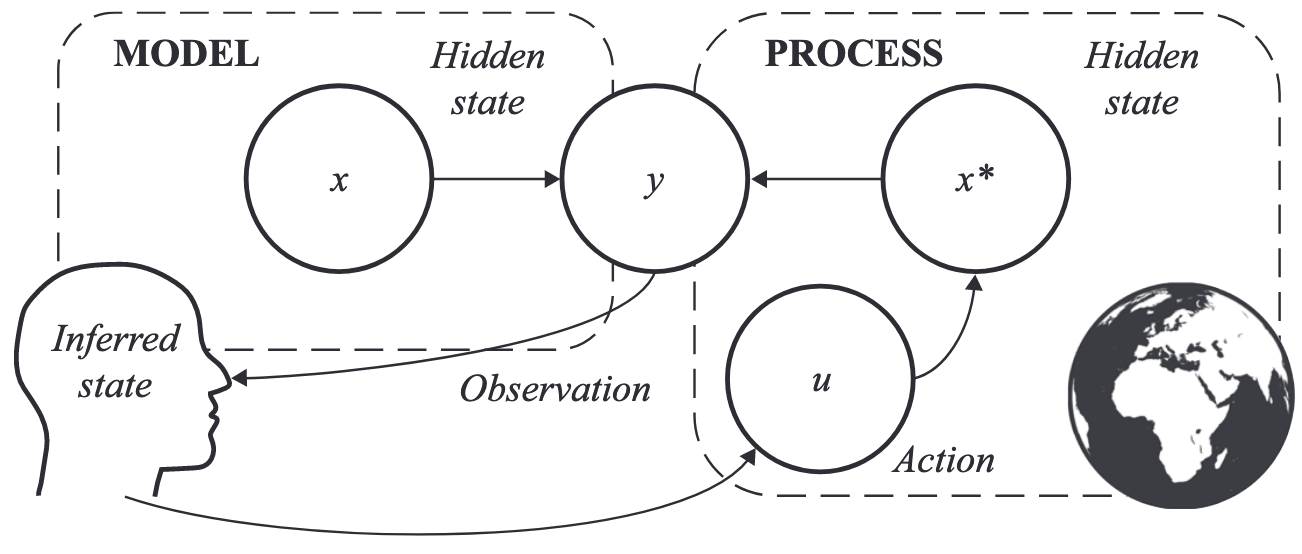
\includegraphics[scale=0.6]{images/generative_process.png}
    \caption{Image from \citet{parr2022ActiveInference} depicting the generative model and process. This depictions shows there are some internal (hidden) parameters of our mode, $x$. Which are inferred by the observations generated by the environment $y$. The central distinction to note is that in theory, there exists some true state of the environment, $x^*$. This is the true causal foundation for observations in the environment. This true state may or may not be with the distribution of states specified by the prior component in the generative model - $P(x)$.}
    \label{fig:generative_process} 
\end{figure}

\subsubsection{Inference and Bayesian Optimality}

So far, we have explored how the brain uses generative models to interpret and predict sensory information. These models allow the brain to integrate top-down expectations (derived from past experiences) with bottom-up sensory input to infer the hidden causes of the world. Now, we can delve deeper into how this inferential process is carried out mathematically, using principles from probability theory - specifically, Bayesian inference. The brain continuously updates its beliefs about hidden states based on incoming sensory data, which can be understood through the lens of Bayes' rule. This formalises the brain's ability to combine prior knowledge with new observations to guide perception and action.

\begin{align}
	\underbrace{P(x | y )}_{\text{Posterior Distribution}} &= \frac{P(y | x)P(x)}{P(y)} \label{eq:posterior} \\
	\underbrace{P(x, y)}_{\text{Generative Model}} &= \underbrace{P(y | x)}_{\text{Likelihood}}\underbrace{P(x)}_{\text{Prior}} \label{eq:decomposed_generative}
\end{align}

\refp{eq:posterior} shows how Bayes' rule updates our beliefs about the hidden states, $x$, given observations, $y$. The posterior distribution, $P(x | y)$, reflects the updated probability of different hidden states after accounting for the new sensory data.

\refp{eq:decomposed_generative} decomposes the generative model into two key components. The likelihood, $P(y | x)$, which expresses how likely the sensory data, $y$, is, given a specific hidden state, $x$. And prior, $P(x)$, which represents our pre-existing beliefs about the hidden states, before observing the new data.

\

Bayesian inference centres on obtaining the posterior distribution, which combines these two components. The term $P(y)$, known as the marginal likelihood or model evidence, serves as a normalizing constant, ensuring that the posterior is a valid probability distribution. In the next section, we will explore the significance of this term and the computational challenges it presents.

\

A few key points about Bayesian inference are worth noting:

\begin{enumerate}
	\item \textbf{Integration of top-down and bottom-up dynamics}: Bayesian inference combines top-down expectations (via the prior) with bottom-up sensory evidence (via the likelihood). This integration echoes the dynamics we previously discussed in the context of perception. The equation $P(x | y) \propto P(y | x) P(x)$ captures this combination of prior knowledge and sensory input, which reflects how the brain balances stored memories and immediate data.
	\item \textbf{Bayesian inference as an optimal process}: In terms of perception and action, Bayesian inference is considered optimal, in the sense that it minimises uncertainty by evaluating the full distribution over hidden states. This optimality becomes particularly important when dealing with uncertainty, as it avoids the shortcomings of approaches that rely solely on single-point estimates.
	\item \textbf{Variational Free Energy (VFE)}: In the context of active inference, Bayesian optimality is achieved by minimising a quantity called variational free energy (VFE), which has roots in statistical physics \citep{friston2006free}. This measure allows the brain to manage uncertainty by aligning its beliefs with the actual sensory data, as we will explore in the next section.
\end{enumerate}

It is essential to emphasise that this optimality is inherently subjective - it depends on the generative model being used. The generative model may or may not capture the true hidden states of the environment, $x^*$, assuming such states exist. In other words, the brain’s model of the world is always limited by its capacity to represent the actual causal dynamics of the environment. If the model fails to include important features of the environment, its predictions will be less accurate. However, Bayesian inference will still be optimal within the bounds of the chosen model. Therefore, the brain’s success in integrating top-down and bottom-up dynamics is constrained by the quality of its generative model.

\subsubsection{Minimising Variational Free Energy}

Having introduced the fundamentals of Bayesian inference, we now turn to two important aspects that were postponed in the previous discussion: the \textbf{marginal likelihood} and \textbf{variational free energy}. These two concepts are intimately connected and central to resolving the challenges that arise in Bayesian inference, particularly when dealing with complex generative models.

\

The fundamental issue with Bayesian inference lies in the computation of the marginal likelihood (or model evidence) in the expression for the posterior distribution \refp{eq:posterior}. In principle, this marginal likelihood is required to normalise the posterior distribution, ensuring that it sums to 1. However, calculating it requires marginalising over all possible hidden states in the generative model:

\begin{equation}
	p(y) = \int p(x, y) \ dx
\end{equation}

This integral sums over the entire state space, which presents two major challenges. 

Firstly, for most real-world models, this integral is too complex to solve \textbf{analytically}. The sheer complexity of generative models, especially in neural processes or high-dimensional spaces, makes exact solutions infeasible. Even when the integral can be approximated numerically, the size of the state space often makes the computation prohibitively expensive. As the dimensionality of the hidden state space increases, the computational cost of evaluating the marginal likelihood grows exponentially

\

To address these issues, we turn to a method known as variational inference. This approach reframes the inference problem as one of optimisation, enabling us to approximate the true Bayesian posterior in a tractable way. The key step in this process is proposing a variational posterior distribution—an approximation to the true posterior that is typically chosen for its simplicity and computational ease. Inference then becomes an optimisation problem with respect to variational free energy (VFE), where the parameters of the variational posterior distribution serve as the adjustable ``levers'' in the optimisation process. By minimising the VFE, we find the best-fitting parameters for the variational posterior, thereby approximating the true posterior as closely as possible. Formally, variational free energy can be defined in terms of the generative model and the variational posterior as follows:

\begin{definition}[Variational Free Energy]\label{def:variational_free_energy}
Let the generative model, $p$, and variational distribution, $q$, be parameterised by $\theta$ and $\phi$ respectively. Then we define variational free energy (VFE) as:
	$$
	\mathcal{F}(q, y) =  \int q(x; \phi) \ln \frac{q(x; \phi)}{p(x, y; \theta)}
	$$
\end{definition}

The claim at the end of the previous section was that Bayesian inference is (subjectively) optimal. Now, having defined variational free energy, we are indeed in a position to demonstrate this.

\begin{equation}\label{eq:vfe_low_road}
	\begin{aligned}
		\mathcal{F}(q, y) &=  \int q(x; \phi) \ln \frac{q(x; \phi)}{p(x, y; \theta)} \\
		&= - \ln p(y; \theta) + \int q(x; \phi) \ln \frac{q(x; \phi)}{p(x | y; \theta)} \\ 
		&= - \underbrace{\ln p(y; \theta)}_{\text{Evidence}} + \underbrace{D_{KL}\left[ q(x; \phi) \,\|\, p(x | y; \theta) \right]}_{\text{Divergence}}
	\end{aligned}
\end{equation}

By Gibbs' inequality, $D_{KL} \geq 0 $, further we can note that if $Q(x; \phi) = P(x | y; \theta)$ then $D_{KL} = 0$. Therefore, is the posterior distribution is the true Bayesian posterior we will be left with negative model evidence. This quantity depends solely on the generative model and not on the inferential process, indicating that Bayesian inference is optimal with respect to VFE and the generative model.

\

However, this does not imply that we cannot further lower the negative log evidence. In fact, one of the fundamental components of active inference is that a system actively engages with its environment. This engagement manifests in the context of VFE, by observing that a system can interact with the environment to create conditions that more closely with its beliefs, thereby minimising the VFE further. This interplay can is depicted in Figure \ref{fig:vfe_minimisation}. 

\begin{figure}[htbp]
    \centering
    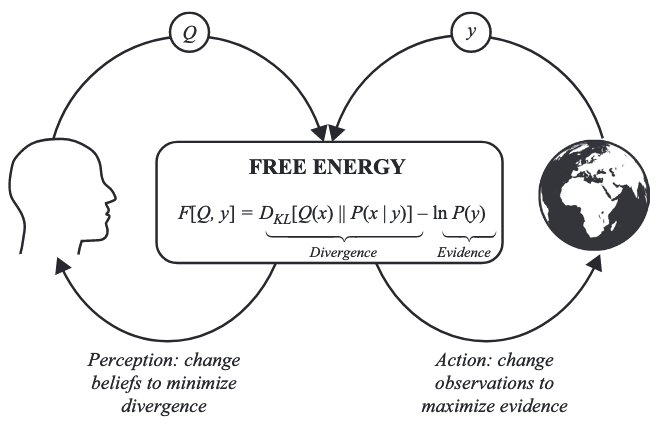
\includegraphics[scale=0.55]{images/vfe_minimisation.png}
    \caption{Image from \citet{parr2022ActiveInference} depicting the interplay between a perception being a process of inference to change beliefs to better reflect the environment, and action as a process to generate observations that better reflect the system's beliefs. In this context, an observations that better suits the beliefs of the model is one with a lower free energy.}
    \label{fig:vfe_minimisation}
\end{figure}

\

The fundamental requirement for Bayesian optimality that we aimed to establish was the interplay between bottom-up and top-down inferential dynamics. These dynamics are indeed reflected in an alternative decomposition of variational free energy (VFE):

\begin{equation}
\begin{aligned}
	\mathcal{F}(Q, y) &=  \int Q(x; \phi) \ln \frac{Q(x; \phi)}{P(x, y; \theta)} \\ 
	&= \underbrace{D_{KL}\left[ Q(x; \phi) \| P(x; \theta)  \right]}_{\text{Complexity}} - \underbrace{\mathbb{E}_{Q(x)}\left[ \ln P(y | x; \theta) \right]}_{\text{Accuracy}}
\end{aligned}
\end{equation}


In this decomposition, we can observe how the two terms map onto the inferential dynamics discussed earlier. The complexity term reflects the degree to which the posterior distribution diverges from the prior beliefs about the hidden states. Minimising this term requires smaller changes to prior beliefs, emphasising bottom-up influences based on past experience.  In contrast, the accuracy term favours internal states that better predict the observed sensory data, thereby promoting top-down processing driven by new sensory stimuli.

\subsubsection{Minimising Surprise}

We have established the link between (approximate) Bayesian inference and top-down and bottom-up inferential dynamics required for perceptual processes. This link was achieved through the use of Variational Free Energy, however this was not the fundamental link we want to establish between Bayesian theories of the brain and active inference. We aim to link these theories to the minimisation of surprise, thus let us define this quantity in terms of the generative model:

\begin{definition}[Surprisal]\label{eq:surprisal}
	$$\mathcal{I}(y) = - \ln P(y)$$
\end{definition}

This definition makes sense with our own notion of surprise. If we believe an observation to be `unlikely', let us say that under our generative model $P(y) = 0.1$, then the surprise of the observation is $ \mathcal{I}(y) \approx 2.3$ nats. \footnote{Like bits, nats are units of information. The choice of unit depends on whether we use a logarithm to the base 2 (bits) or a natural logarithm (nats).} While, say $P(y) = 0.8$ then $\mathcal{I}(y) \approx 0.1$ nats. 

\

We can notice that we have already shown that the process of Bayesian inference does indeed seek to minimise surprise:

\begin{equation}
	\begin{aligned}
		\mathcal{F}(Q, y) &= - \ln P(y; \theta) + D_{KL}\left[ Q(x; \phi) \| P(x | y; \theta) \right] \\
		&\geq - \ln P(y; \theta) \\
		&= \mathcal{I}(y)
	\end{aligned}
\end{equation}

This demonstrates is that VFE is an upper bound on surprise. Therefore, the minimisation of VFE will result in the minimisation of surprise. Further, as we argued in the previous section, minimising VFE can be done by changing our beliefs to better reflect the environment, as well as changing the environment to reflect our beliefs. These are the conditions that we required to justify the brain performing active inference. 

\subsubsection{Expected Free Energy}

While we have justified the brain's engagement in active inference, we must also recognise a fundamental \textit{prospective} aspect of cognition that we have not mentioned as of yet: \textit{planning}.

\

Within active inference, planning is similarly treated as an inferential process. To align with the Bayesian approach we have followed we must define priors and likelihoods. These distributions will be over \textit{policies}. In active inference, a sequence of actions is referred to as a \textit{policy}. It is important to distinguish between actions, which directly influence the external world, and policies, which represent behaviour patterns.

\

Future observations resulting from a particular policy are unknown, as they have not yet occurred, and must be predicted by the generative model. This prediction relies on two components: first, our belief about how hidden states evolve under a policy, denoted by $p(\tilde{x} | \pi)$, where $\tilde{x}$ represents a trajectory of hidden states. Second, the likelihood distribution, $p(y | x)$, describes the expected observations given hidden states. These two components enable the brain to simulate the counterfactual consequences of its actions, akin to asking: ``What happens if I do this?'' By marginalising over hidden states, we obtain the marginal likelihood (or its free energy approximation), $p(\tilde{y} | \pi)$, which reflects the evidence for a policy.

\

Active inference breaks planning into two steps: first, assigning a score to each policy, and second, forming posterior beliefs about which policy to pursue. The prior belief about which policy to follow depends on its score, where better policies are assigned higher probabilities. In active inference, the score of a policy is the negative \textit{expected free energy}, $\mathcal{G}$, which is similar to variational free energy, except for the constraint that observations too need to be treated as random variables.

\subsubsection{Computing EFE}

We have assumed that during planning, the organism scores its policies according to their expected free energy. However, we have not yet defined what expected free energy is:

\begin{equation}\label{eq:efe}
	\begin{aligned}
		\mathcal{G}_\pi &= \int Q(\tilde{x}, \tilde{y} | \pi) \ln \frac{Q(\tilde{x} | \pi)}{P(\tilde{x}, \tilde{y} | \pi)} & \text{(L1)}\\ 
		&= \mathbb{E}_{Q(\tilde{x}, \tilde{y} | \pi)} \left[ \ln \frac{Q(\tilde{x} | \pi)}{P(\tilde{x}, \tilde{y} | \pi)} \right] & \text{(L2)} \\
		&\approx \mathbb{E}_{Q(\tilde{x}, \tilde{y} | \pi)} \left[ \ln Q(\tilde{x} | \pi) - \ln Q(\tilde{x} | \tilde{y}, \pi) \right] - \mathbb{E}_{Q(\tilde{y} | \pi)}\left[ \ln P(\tilde{y} | C) \right] & \text{(L3)}\\
		&= - \underbrace{\mathbb{E}_{Q(\tilde{x}, \tilde{y} | \pi)} \left[ \ln Q(\tilde{x} | \tilde{y}, \pi) - \ln Q(\tilde{x} | \pi) \right]}_{\text{Epistemic}} - \underbrace{\mathbb{E}_{Q(\tilde{y} | \pi)}\left[ \ln Q(\tilde{y} | C) \right]}_{\text{Pragmatic}} & \text{(L4)}\\ 
	\end{aligned}
\end{equation}


The definition of EFE in (L1) is identical to the definition of VFE in \refp{eq:vfe_low_road}, except for the first variational posterior distribution term including the observations as well as $\tilde{x}, \tilde{y}$ representing a trajectory. The observations can then enter the expectation in (L2). This makes sense since we are considering observations that have not occurred yet. (L3) is a fundamental step in active inference, first we replace the true posterior with our variational posterior ($P(\tilde{x} | \tilde{y}, \pi) \to Q(\tilde{x} | \tilde{y}, \pi)$). Second, we drop the condition on $\pi$ in the second term, instead we condition on some distribution that is used to encode the preferences of the system, $C$. This means the system seeks to find policies expected to produce those observations. The agent’s preferences can be independent of the policy being followed, which allows us to drop the condition on $\pi$. 

\

(L4) labels two terms that underscore active inference's appeal in planning. The first term is the epistemic term, notice that this term is negated, thus to minimise EFE, we need to maximise this epistemic term. What this term is representing is the difference between the variational distribution prior and conditional on an observation. That is - the agent is driven to seek out observations that reduce uncertainty about hidden states \citep{smith2022} The second term is the pragmatic term which as mentioned allows us to score the observations with respect to the agent's preferences. 

\section{Applications} 

In this section, we move from the conceptual foundation of active inference to its practical applications, aiming to demonstrate how active inference, alongside other computational neural models, can be applied to planning and control problems. This marks a shift from the previous discussion, which focused on active inference as a theoretical framework without direct empirical validation. Here, we explore the \textit{process theories} that propose neural implementations of the computations central to active inference.

\

Process theories are crucial for understanding how the abstract principles of active inference can be realised within neural systems. These theories suggest that neural networks implement inference by propagating locally computed messages between neurons, constrained by the network's structure and synaptic connections \citep{parr2019neuronal}. This imposes specific limitations on the kinds of models that can be employed. For example, traditional multi-layer perceptrons trained via backpropagation require a global error signal, which is incompatible with the localised, synapse-driven computations hypothesised by process theories. Instead, we will focus on models like predictive coding and message-passing algorithms, which respect these constraints and offer a more biologically plausible framework for active inference.

\

All of the environments we consider will be framed as Markov decision processes (MDPs), a common formalism for modelling decision-making under uncertainty. Before discussing neural implementations, it is important to briefly review the key aspects of MDPs, as they provide the mathematical foundation for the problem that will be discussed later on in this section.

\paragraph{Markov Decision Processes}

A Markov Decision Process (MDP) is a mathematical framework used to model decision-making problems where outcomes are both under the control of the agent and subject to stochastic influences. An MDP consists of a set of states, actions, transition probabilities, and rewards. At each time step, the system occupies a particular state, and the agent selects an action. This action results in a transition to a new state, according to a probability distribution that models the system’s dynamics. While classical MDPs aim to maximise expected cumulative rewards, in active inference, the objective is reframed as minimising free energy. This subtly shifts the focus from direct reward maximisation to ensuring that the agent’s beliefs and sensory observations remain consistent with its internal model of the world.

\

A key feature of MDPs is the \textit{Markov property}, which ensures that the future state depends only on the current state and action, not on the sequence of past states or actions. This leads to a \textit{Markov chain} over the hidden states, where the evolution of the system can be fully described by its current state and transition probabilities.

\paragraph{Observations and Hidden States: MDPs vs. POMDPs}

In standard MDPs, the agent has full access to the current state of the system, allowing it to make decisions based directly on this information. However, real-world environments often involve uncertainty or partial observability, which brings us to a distinction between MDPs and Partially Observable Markov Decision Processes (POMDPs).

\

\textbf{MDP}: In an MDP, the agent has full observability, meaning it knows the exact state of the system at each time step. Decisions are made based on the current state, and the transitions form a fully known Markov chain.

\

\textbf{POMDP}: By contrast, a POMDP introduces the concept of hidden states—underlying states that are not directly observable by the agent. Instead of receiving perfect state information, the agent receives noisy or incomplete observations, which it must use to infer the true hidden state. This inference is typically performed by maintaining a belief state—a probability distribution over possible hidden states. The agent’s decisions must therefore account not only for the underlying dynamics of the hidden states but also for the uncertainty inherent in the observations.

\

The distinction between MDPs and POMDPs is crucial for modelling real-world decision-making tasks. While MDPs are suited to environments where the agent can directly access the state, POMDPs are more appropriate for scenarios where the agent must infer hidden states from noisy data, such as in robotic control, navigation, or decision-making under uncertainty in biological systems. This added complexity makes POMDPs a natural fit for active inference models, as they align with the uncertainty and belief-updating processes that are central to minimising free energy.

\subsection{Predictive Coding}\label{section:predictive_coding}

We now transition our implementation of active inference into continuous state spaces by presenting an active inference agent equipped with a generative model inspired by \textit{predictive coding}. This section will differ somewhat from other implementations in this report, adopting a tutorial-style approach similar to that presented by \citet{bogacz2017tutorial}.

\

Predictive coding presents a theory of cortical function - namely, that the core function of the brain is to minimise prediction error. The intuition behind this is that the brain is comprised of a hierarchy of neurons making predictions about the activity of the neurons in the level below them. \citep{friston2008hierarchical} The prediction error in this case is the difference between the neural activity predicted by the higher level compared to the actual neural activity. Over time, the hierarchy of layers encodes a range of predictions at difference scales, with fine details in local sensory data represented at the lower levels and global invariant properties of the causes of sensory data encoded at higher levels \citep{millidge2021applications}. 

\

These prediction errors are propagated up the hierarchy and used to improve future predictions. In predictive coding, there are two main strategies for reducing prediction errors. The first is immediate inference about the hidden states of the world, akin to perception. In this process, the prior predictions of a layer are updated by integrating residual errors from the layer below, following principles of Bayesian inference. This is performed through variational inference, where the brain iteratively updates its beliefs about hidden states by minimising free energy.

\

Secondly, though updating the model of the world to better explain the sensory data, which corresponds to learning. Synaptic connections between neurons, characterised by synaptic weights, are adjusted based on prediction errors. These adjustments modulate the strength of connections between neurons, allowing the brain to refine its predictions about lower-level neural activity.

\subsubsection{Origins}

The origins of predictive coding as a neuroscientific theory trace back to the 1980s and 1990s, with \citet{rao1999predictive} being one of the seminal papers introducing predictive coding as a model of neural processing. In this study, predictive coding was applied to visual processing, where a hierarchical network of neurons was exposed to natural images. The model's neurons developed simple-cell-like receptive fields, while those encoding prediction errors\footnote{The term ``predictive coding'' stems from the fact that certain nodes in the model explicitly encode these prediction errors} exhibited end-stopping and other extra-classical receptive-field effects \citep{rao1999predictive}.

\

Predictive coding, in its fully developed mathematical form, was later extended by \citet{friston2003learning, friston2005theory}, who linked the minimisation of prediction error to the minimization of free energy within the expectation-maximisation framework \citep{dempster1977maximum}. This formulation unified predictive coding with the broader concept of free energy minimisation, as we will explore in more detail in subsequent sections.

\subsubsection{Predictive Coding as Variational Inference}

The modern implementation of prediction coding can be best understood as a variational inference algorithm \citep{millidge2021applications}. Meaning that the predictive coding algorithm defines a generative model, comprising of a prior and a likelihood distribution. In the case of predictive coding these distributions are Gaussian. Further, variational inference requires a variational posterior distribution that is used as the tractable approximation to the Bayesian posterior. Let us define these components for our model.\footnote{We are assuming a single hidden state and a single observation dimension for this section. Hence we define the variance as a scalar value - $\sigma^2$ - , rather than as a matrix - $\Sigma$ - which will be done. Similarly, $x$, $y$ represent scalar values and not vectors. }

\begin{equation}\label{eq:pc_single_model}
    \begin{aligned}
        & q(x ; \phi) = \delta( x - \phi ) &(A) \\
        & y | x \sim N(f(x	; \theta), \sigma^2_y) &(B) \\
        & x \sim N(\bar{\mu}, \sigma^2_x) &(C) \\ 
    \end{aligned}
\end{equation}

(A) - This is our variational posterior distribution. $\delta$ denotes the Dirac-delta distribution which is a point mass probability distribution. The alternative form of the variational posterior is a Gaussian under the Laplace approximation. \cite{friston2003learning} This approximation defines the variance of a Gaussian distribution as a function of its mean. Essentially, allowing us to focus solely on estimating the first moment of the distribution. Both of these forms results in the same variational inference update equations and thus we have chosen the Dirac-delta for simplicity. Predictive coding under the Laplace approximation will be derived in Appendix \ref{appendix:laplace_approx}. 

\

(B) - This is the form of our likelihood distribution. This component represents the beliefs the model has about how sensory observations, $y$, are generated from the hidden state of the model $x$. We are assuming the relation is some function $f$ of the hidden states parameterised by $\theta$. As well as variance $\sigma_y^2$

\

(C) - This defines the form of our prior beliefs about the hidden variable of our model, $x$. In this case, it is defined as a Gaussian with a mean of $\bar{\mu}$. We will be assuming a value of this when we operationalise this model.

\

The model components that are needed for inference have been defined, let us now consider an alternative decomposition of VFE that is more convenient for the derivations of the update equations in variational inference:

\begin{equation}\label{eq:vfe_entropy_energy}
	\mathcal{F} = \underbrace{\mathbb{E}_{q(x ; \phi)} \left[ 	\ln q(x ; \phi) \right]}_{\text{Entropy}} - \underbrace{\mathbb{E}_{q(x ; \phi)} \left[ 	\ln p(y | x ; \theta) p(x) \right]}_{\text{Energy}} \\
\end{equation}


This is a useful form since we need only consider the energy term since the entropy of a Dirac-delta distribution is 0.

\begin{equation}\label{eq:pc_vfe}
	\begin{aligned}
	& \mathbb{E}_{q(x ; \phi)} \left[ 	\ln p(y | x ; \theta) p(x) \right] \\
	&= \int \delta(x - \phi) \ln \left( \mathcal{N}(y ; f(x; \theta), \sigma^2_y) \ \mathcal{N}(x; \bar{\mu};, \sigma^2_x) \right) dx \\
		&= \ln \mathcal{N}(y; f(\phi; \theta), \sigma^2_y) + \ln \mathcal{N}(\phi; \bar{\mu}, \sigma^2_x) \\
		&= - \frac{(y - f(\phi; \theta))^2}{\sigma^2_y} - \ln 2 \pi \sigma^2_y - \frac{(\phi - \bar{\mu})^2}{\sigma^2_x} - \ln 2 \pi \sigma^2_x \\
		&= - \frac{1}{2}\left[ \epsilon_y^2 + \epsilon_x^2 +\ln 2 \pi \sigma^2_y +\ln 2 \pi \sigma^2_x  \right]
	\end{aligned}
\end{equation}

Where, $\epsilon_y := \frac{y - f(\phi; \theta)}{\sigma_y}$ and $\epsilon_x := \frac{\phi - \bar{\mu}}{\sigma_x}$ are the prediction errors that we have reference in the predictive coding model. 

\

This expression shows that not all errors are equal \citep{hodson2023empirical}. These errors are weighted by their respective standard deviation. Meaning errors with relatively higher deviation will have reduced effect on our free energy term. Anthropomorphising this, if we have a high degree of uncertainty about something we see, we tend to now take it as seriously as if we absolutely sure it is true. This is an important feature in models where the variance is treated as a model parameters to be learnt, \citep{bogacz2017tutorial, friston2003learning} however we will not be considering this in our current model.

\

To operationalise the variational inference we will be taking the partial derivatives of the variational free energy. So let us put \refp{eq:pc_vfe} and \refp{eq:vfe_entropy_energy} together to make the optimisation objective clear:

\begin{equation}\label{eq:vfe_pc}
	-\mathcal{F} = \frac{1}{2}\left[ \epsilon_y^2 + \epsilon_x^2 +\ln 2 \pi \sigma^2_y +\ln 2 \pi \sigma^2_x  \right]
\end{equation}

We have negated the VFE since we aim to minimise this. 

\

The final assumption that needs to be made is that variational free energy can be minimised using the method of gradient descent such that:

\begin{equation}
	\frac{d \phi}{dt} = -\frac{\partial \mathcal{F}}{\partial \phi}
\end{equation}

This key assumption governs the temporal dynamics of the hidden variable. It implies that the hidden state will evolve to minimize the prediction error over time, reflecting an essential principle of predictive coding.

\

Using this assumption, we can take the partial derivative of \ref{eq:vfe_pc} with respect to the variables of interest:

\begin{equation}\label{eq:pc_update_equations}
	\begin{aligned}
		\frac{d \phi}{dt} &= -\frac{\partial \mathcal{F}}{\partial \phi} = \epsilon_y \frac{\partial f(\phi, \theta)}{\partial \phi} - \epsilon_x, \\
    \frac{d \theta}{dt} &= - \frac{\partial \mathcal{F}}{\partial \theta}  = \epsilon_y \frac{\partial f(\phi, \theta)}{\partial \theta}
    \end{aligned}
\end{equation}

These update rules define our algorithm for conducting variational inference. A subtle consideration here is balancing the updates of the variational posterior parameter $\phi$ (representing the hidden state estimate) and the generative model parameter $\theta$ (representing the mapping from hidden states to observations). From a neurobiological perspective, $\phi$ corresponds to changes in neural activity, while $\theta$ reflects changes in synaptic weights. The balance between updating these variables is critical for ensuring efficient inference. From a statistical perspective, this balance can be managed using methods such as expectation maximisation.

\subsubsection{Expectation Maximisation}

Expectation-Maximisation (EM) provides a well-established procedure for the estimation of probability densities \citep{friston2003learning}. The algorithm alternates between two steps: the Expectation (E) step and the Maximisation (M) step. In the E step, the expected values of the hidden variables are computed given the current model parameters. In the M step, the likelihood of the observed data is maximized with respect to the model parameters. Both steps are performed with respect to the same objective function—variational free energy \citep{friston2003learning}.

\

Typically, these dynamics involve fully relaxing the system with respect to the hidden variables during the E step, allowing them to reach an equilibrium. Afterward, in the M step, the system relaxes again, this time with respect to the parameters $\theta$, to maximize the likelihood. However, in our model, we take a slightly different approach. Neural activity typically operates on a much faster timescale than synaptic weight changes \citep{millidge2024temporal}. Thus, while we retain the full relaxation during the E step, we modify the M step by taking only a single gradient descent step on the parameters $\theta$, instead of fully relaxing the system.

\

There are alternative approaches to minimising variational free energy within predictive coding models. For example, \citet{song2020can} propose adjusting synaptic weights at specific intervals during the relaxation of neural activity. This approach was used in the context of approximating backpropagation in predictive coding networks. Furthermore, \citet{salvatori2024a} show that alternating gradient descent steps between the weights and the hidden states can result in both fast and stable inference in predictive coding networks. However, this was applied to large hierarchical predictive coding models which fall outside the scope of the present example. For the purposes of this report, we will adopt the standard EM-like scheme, of complete relaxation with respect to the neural activity, and then a single step with respect to the synaptic weight.

\subsubsection{Bayesian Thermostat}

We are now in a position to demonstrate the predictive coding algorithm. The environment we will be considering is the Bayesian Thermostat, as described by \citet{buckley2017free}. In this environment, an agent observes the temperature from a heat source. The agent’s observations, denoted as $y$, correspond to temperature readings. The hidden state, $x$, represents the distance between the agent and the heat source.

We assume that the true causal structure governing the temperature readings as a function of distance is given by:

\begin{equation}\label{eq:bayesian_thermostat}
	y = 10 - x
\end{equation}

That is, the temperature decreases linearly as the agent moves away from the heat source. Additionally, we assume the agent receives noisy temperature readings. The relationship between temperature and distance, incorporating this noise, is modelled as:

\begin{equation}
	y = 10 - x + \omega, \quad \omega \sim N(0, \frac{1}{25})
\end{equation}

Here, $\omega$ represents Gaussian noise with mean zero and variance $\frac{1}{25}$, reflecting uncertainty in the agent's temperature observations.

\begin{figure}[htbp]
    \centering
    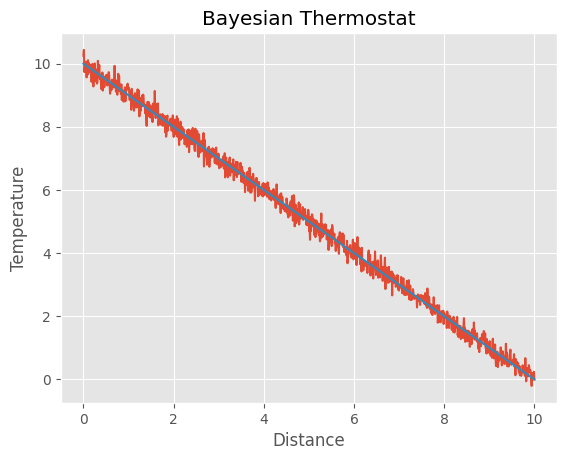
\includegraphics[scale=0.55]{images/bayesian_theromostat.png}
    \caption{Visualisation of the Bayesian Thermostat environment with the true line depicting the line $y = 10 - x$. While the red is a demonstration of the type of observations the agent would receive in the environment.}
    \label{fig:bayesian_thermostat}
\end{figure}

\subsubsection{Perception}

The problem of perception within the Bayesian Thermostat environment is inferring the distance the agent is from the heat source, given the noisy temperature readings generated by the environment. To demonstrate this we will need to set the parameters of the generative components mentioned previously.

\begin{equation}\label{eq:bayesian_thermostat_generative_model}
	\begin{aligned}
		y | x &\sim N\left(f(x), \frac{1}{16}\right), \  x &\sim N\left(\bar{\mu}, \frac{1}{16}\right) ,\ f(x) &= 10 - x
	\end{aligned}
\end{equation}

Here, $y | x$ represents the temperature readings conditioned on the hidden state $x$, and $f(x)$ captures the functional relationship between the temperature and distance.

\

Note the distinction between $f$, a component of the generative model, and the underlying causal structure of the data-generating process, defined earlier in \refp{eq:bayesian_thermostat}. For the purpose of perception, we assume that $f$ accurately describes this underlying relationship. Furthermore, $f$ here is solely a function of the neural activity (or hidden state) $x$ and not the synaptic weights, as we are not yet considering learning; this will be treated in the next section.

\

\paragraph{Remark} Although it is formally a function of the hidden state $x$, during inference, we will treat it as a function of $\phi$, the posterior belief about $x$. This is natural since we are inferring the posterior value of $x$ through iterations on $\phi$.

\

The final component of our generative model is the variational posterior distribution, we will be assuming this takes the form of a Dirac-delta distribution centred at $\phi$. Thus, can now derive the update equations for the hidden variable during inference in the Bayesian Thermostat environment from \refp{eq:pc_update_equations}: 

\begin{equation}\label{eq:pc_perception_phi}
	\begin{aligned}
		\frac{d \phi}{dt} = -\frac{\partial \mathcal{F}}{\partial \phi} &= \epsilon_y \frac{\partial f(\phi)}{\partial \phi} - \epsilon_x \\
		&= -\epsilon_y - \epsilon_x \\
    \end{aligned}
\end{equation}

During simulation we will update this hidden state using Euler's method, meaning we have some step size $\tau$ that is used to perform gradient on the VFE:

\begin{equation}
	\phi_{k + 1} = \phi_{k} + \tau \left( - \epsilon_y - \epsilon_x \right) 
\end{equation}

\paragraph{Remark} A point to note here is the different temporal scales we have introduced. $k$ denotes the time corresponding to the inference steps in the numerical implementation. Meaning that after convergence we update the hidden state for the environment time $t$. Precisely:

\begin{equation}
	x_{t + 1} = \phi_K
\end{equation}

Where $K$ denotes the inference steps that were needed for convergence. Which is a hyperparameter for the model set at 10 in this case.

\

Suppose the agent's prior belief of its distance to the heat source, $\bar{\mu}$, is $4$. Meaning that the agent is expecting to observe a temperature reading of $f(4) = 6$. While further assume that the agent actually receives a temperature reading of $y = 2$. Meaning that it is likely that the agent is further from the heat source than its prior beliefs dictate. Indeed this is reflected in a plot of the inference steps in Figure \ref{fig:pc_example_perception}.

\begin{figure}[h]
    \centering

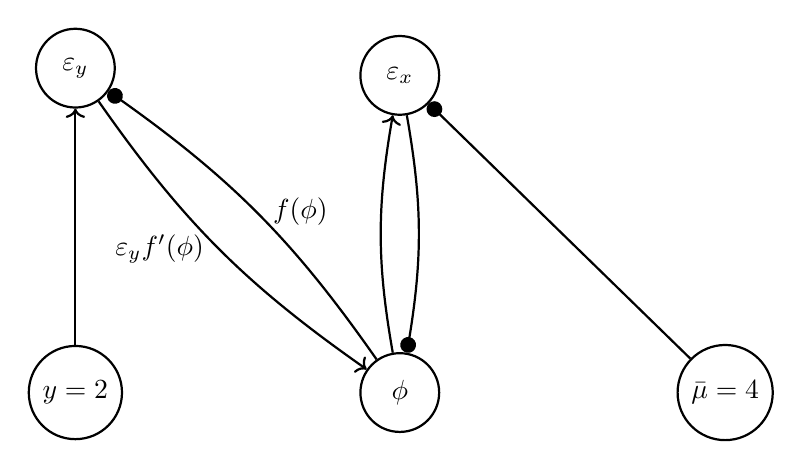
\begin{tikzpicture}[node distance=3cm, auto, thick, 
    every node/.style={circle, draw, minimum size=1cm}, 
    every path/.style={draw}]
	
	%Nodes
    \node (y) at (0,0) {$y = 2$};    
    \node (eps_y) [above=of y] {$\varepsilon_y$};
    \node (phi) [right=of y] {$\phi$};
    \node (eps_x) [above=of phi] {$\varepsilon_x$};
    \node (prior) [right=of phi] {$\bar{\mu} = 4$};

    % Edges
    \draw[->] (y) to  (eps_y);
    \draw[->, bend right=10] (eps_y) to node[midway, left, draw=none] {$\varepsilon_y f'(\phi)$} (phi);
    \draw[-{Circle[length=2mm]}, bend right=10] (phi) to node[midway, right, draw=none] {$f(\phi)$} (eps_y);
    \draw[->, bend left=10] (phi) to (eps_x);
    \draw[-{Circle[length=2mm]}, bend left=10] (eps_x) to (phi);
    \draw[-{Circle[length=2mm]}] (prior) to (eps_x);
    
\end{tikzpicture}
\caption{The architecture of the predictive coding model that is used in the perception task in the Bayesian Thermostat environment. Lines with arrows denote excitatory connections while lines ended with circles denote inhibitory connections. Lines with no labels denote a weight of 1.}
\label{fig:pred_coding}
\end{figure}

\begin{figure}[htbp]
    \centering
    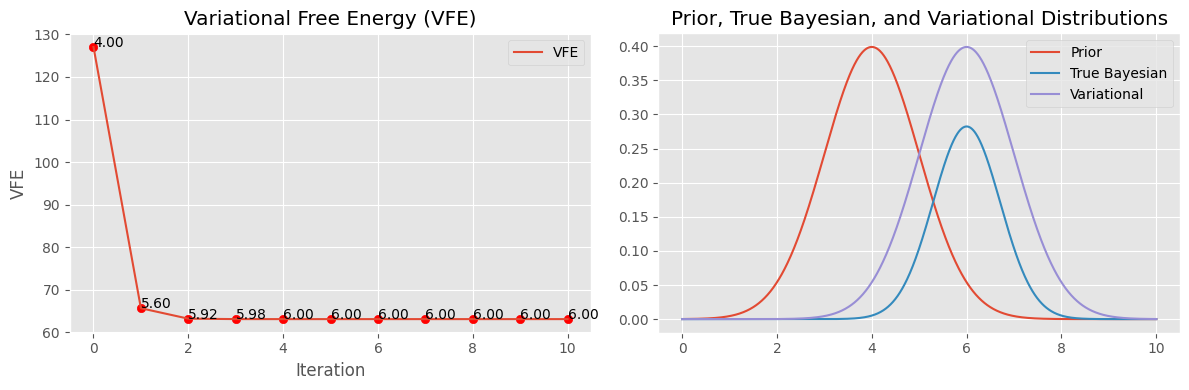
\includegraphics[scale=0.55]{images/pc_example_perception.png}
    \caption{\textbf{Left}: Plot of the the values of VFE during gradient descent. Each value plotted corresponds to the value of $\phi$ used in the calculation of the VFE. \textbf{Right}: After convergence of the $\phi$ we then use the parameter as the mean of our prior term in the generative model. This plot shows the difference between the prior distribution, the variational posterior and the true Bayesian posterior distribution. Important to note is that we are only performing gradient descent on the $\phi$ and simply keeping the variance of the prior distribution constant after convergence.}
    \label{fig:pc_example_perception}
\end{figure}

\

What we note about the inference plot in Figure \ref{fig:pc_example_perception} is that the variational posterior distribution does indeed correctly infer the true Bayesian posterior mean. The difference between these two distribution is due to the fact that we are not learning the variance of these distributions. You can refer to \citet{bogacz2017tutorial, friston2003learning} for demonstrations on this. It is also interesting to note for those not familiar with Bayesian inference, how the new posterior mean of the distribution over hidden states is not the value that best describes the data, which in this case would be $x = 8$. But, the posterior beliefs represent a tradeoff between this optimal update and the priors beliefs about the hidden states.

\subsubsection{Learning}

We now aim to relax some of the assumptions that were made in the perception section. Namely, we will not assume that the agent has a perfect representation of the causal dynamics of the environment ie. we will assume that $f$ does not perfectly describe the relationship between the distance and the temperature. We will assume this function has the following form:

\begin{equation}
	f(x, \theta) = 10 - \theta x
\end{equation}

Practically, this means the model is required to not only infer where in the environment they are, but only learn the relation between where they are and the temperature. This is indeed somewhat circular, we require the dynamics to accurately infer where we are, but we need to know where we are to accurately infer the dynamics. This is the essential problem we are trying to solve. 

\

To learn and update the synaptic weights we will similarly use \refp{eq:pc_update_equations} to derive our update equations for $\theta$:

\begin{equation}\label{eq:theta_gradient_descent}
	\begin{aligned}
		\frac{d \theta}{dt} = - \frac{\partial \mathcal{F}}{\partial \theta}  &= \epsilon_y \frac{\partial f(\phi, \theta)}{\partial \theta} \\
		&= \eta \theta \epsilon_y
	\end{aligned}
\end{equation}

$\eta$ is the learning rate of the model, which controls the size of the update step for the synaptic weights. This is a common parameter in neural network training and is crucial for regulating the gradient descent process. The reason for constraining the update step is that the objective surface with respect to the synaptic weights is often non-linear and not well-behaved, meaning large updates could lead to instability or poor convergence. Therefore, $\eta$ helps ensure smoother and more controlled updates.

\

In this example, the learning rate is set to $0.01$, which is a hyper-parameter that must be tuned based on the specific problem. We will use Euler’s method to update the synaptic weights as follows:


\begin{equation*}
	\theta_{t + 1} = \theta_{t} + \tau ( \eta \phi \epsilon_y )
\end{equation*}

Notice that this temporal scale is the environment's. Meaning that we will take a single gradient descent step with respect to the weight. We will also need to adjust the algorithm for hidden state inference given the generalisation of $f$:

\begin{equation}\label{eq:pc_learning_phi}
	\begin{aligned}
		\frac{d \phi}{dt} = -\frac{\partial \mathcal{F}}{\partial \phi} &= \epsilon_y \frac{\partial f(\phi, \theta)}{\partial \phi} - \epsilon_x \\
		&= \theta \epsilon_y - \epsilon_x \\
    \end{aligned}
\end{equation}

We assume the same prior and observation as the previous section. Only that we are now required to initialise the $\theta = -0.75$. We see the results from the inference scheme in \ref{fig:pc_example_learning}. 

\

\begin{figure}[htbp]
	\centering
	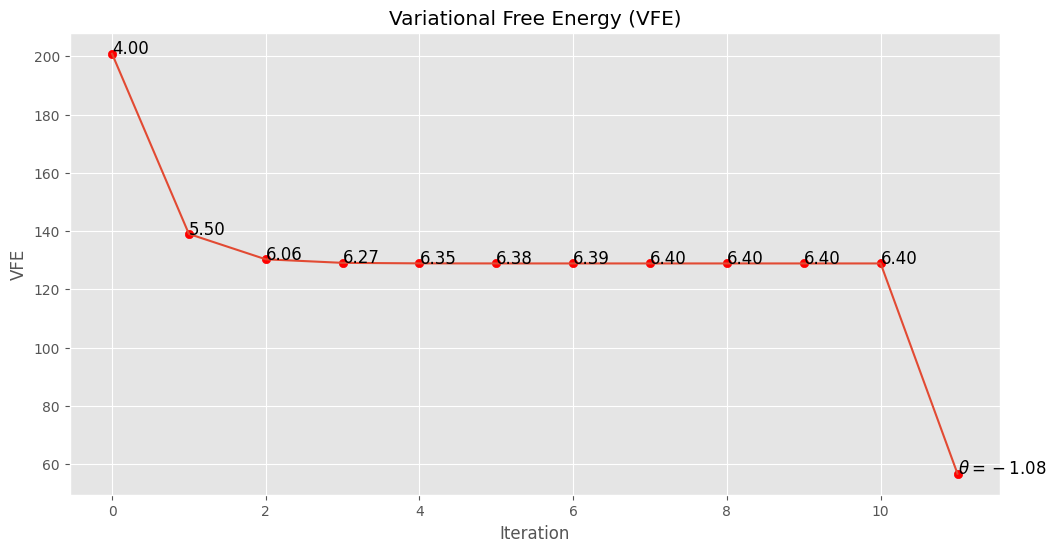
\includegraphics[scale=0.5]{images/pc_example_learning.png}
	\caption{The gradient descent on VFE that was described in the example of learning in predictive coding. The first 10 points demonstrate the descent with respect to $\phi$ and the final step is the step with respect to $\theta$ described in \refp{eq:theta_gradient_descent} With hyper-parameters of $\eta = 0.01$ and $\tau = 0.01$} 
	\label{fig:pc_example_learning}
\end{figure}

We observe that the variational free energy (VFE) converges to a value higher than that seen in Figure \ref{fig:pc_example_perception} in the perception section. However, the maximisation step (M-step) in the expectation-maximisation (EM) scheme brings the VFE below what was observed during perception alone. Interestingly, this update with respect to $\theta$ actually overestimates the synaptic weight (-1.08 compared to the true value of -1). This is not surprising given that the inferred hidden distance converges to 6.4. As a result, the temperature readings are better explained by a larger $\theta$ based on the model’s prior beliefs, leading to an overestimation of the true value.

\

This outcome demonstrates how inference is constrained by the model's ability to explain the environment. Since the agent is mistaken about both its distance from the heat source and its belief about the relationship between distance and temperature, it is natural to observe instability in the inference process. These inaccuracies reflect how the model's underlying assumptions can cause deviations from the true values during the learning process.

\subsubsection{Planning}

The final form of cognition in our predictive coding model is planning. Up to this point, we have focused on perception and learning without explicitly referring to active inference. However, as seen in the previous sections, variational free energy minimisation is closely related to the principles of active inference. Predictive coding, as described so far, does not inherently involve planning. To introduce planning, we will leverage the expected free energy (EFE) functional to define distributions over policies.

\

In this context, we will consider a single time-step into the future, which is sufficient for planning within the simplicity of this environment.

\

The simplification that is made in this model of planning is the transitions. We will assume that the agent knows exactly how (its beliefs) of the distance to the heat source will change with each action. We define 3 actions that the agent can take: Left, right and stay. Further, we define the transition dynamics as Dirac-delta distributions:

\begin{equation}
\begin{aligned}
	P(x_{t+1} | x_t, u^S_{t+1}) &= \delta(x_{t+1} - x_t ) \\
	P(x_{t+1} | x_t, u^L_{t+1}) &= \delta(x_{t+1} - ( x_t - 0.01) ) \\
	P(x_{t+1} | x_t, u^R_{t+1}) &= \delta(x_{t+1} - ( x_t + 0.01) ) 
\end{aligned}
\end{equation}

Where $u^L$ is the move left action, $u^S$ is stay and $u^R$ is move right. These transitions mean that the agent will move 0.01 units right when the right action is taken. Similarly, for the left action. And will stay at the sample place with the stay action. 

\

As described in the previous section, the EFE is evaluated based on some preference distribution over actions. In this way we allow for the agent to be goal-directed. For this environment, we will again assume that the preference distribution is a Gaussian distribution over the observations:

\begin{equation}
	y | C \sim N(4, \frac{1}{16})
\end{equation}

This preference is completely arbitrary and is defined for demonstration. But we are now able to use these components to define the expected free energy for each action. We will be choosing an alternative expression for the functional than what we saw in \refp{eq:efe} for ease of computation:

\begin{equation}\label{eq:efe_thermostat}
	\mathcal{G}(u_{t+1}) = \underbrace{\mathbb{E}_{Q(x_{t+1} | u_{t+1})} \left[ H[ P(y_{t+1} | x_{t+1}) ] \right]}_{\text{Ambiguity}} + \underbrace{D_{KL}\left[ Q(y_{t+1} | u_{t+1} \| P(y_{t+1} | C)) \right]}_{\text{Risk}}
\end{equation}

Let us now discuss each of these terms of how they are implemented in our scheme.

\

Ambiguity - This expression for EFE is particularly useful for Gaussian generative models since the entropy ($H(\cdot)$) of a normal distribution is only a function of the variance of the distribution not the mean. Since we are only considering learning of the mean this term becomes constant. Nevertheless, we have kept this term within the model since it will encourage exploration within the agent. This will become more clear when we demonstrate how exactly we create a distribution over the policies using EFE.

\

Risk - This is our expected divergence between the next observation and our preference distribution.

\

The EFE `values' each policy we are able to undertake, however, since we are assuming planning is as inference we will want to be able to sample from a distribution over the policy values to choose which action to take. To do this we will apply the softmax ($\sigma(\cdot)$) function to convert the EFE values for each policy into a distribution:

\begin{equation}
	P(\textbf{u}_{t+1}) = \sigma( - \mathcal{G}(\textbf{u}_{t+1}) )
\end{equation}

The softmax function will scale the vector input of actions into a distribution of actions proportional to the negative EFE. This makes sense since our aim is to minimise free energy. This is the why we have kept in the ambiguity constant, since this will increase the EFE of all actions equally it essentially saturates the relative expected free energy of each action. Which in some instances may be detrimental to the performance of the model. However, we have found that this term allowed for more diverse actions selection initially which meant the agent learnt the dynamics of the environment in a more efficient way.

\

What we aim to demonstrate with planning is that the agent is able to consistently observe preferable temperature readings even in a noisy environment. What this means is that we need to dynamics of the agent to evolve over more than just a single time-step, which has been the approach to the tutorial thus far.

\

We have kept prior knowledge of distance consistent with prior sections, but we have set the true distance the agent is from the heat source as 8.\footnote{We have included a table of hyperparameters for this section and all previous section in Appendix \ref{appendix:hyperparameters}.} And allowed the agent to interact with the environment for 250 time-steps, with the results plotted in \ref{fig:pc_example_planning}. 

\begin{figure}[htbp]
	\centering
	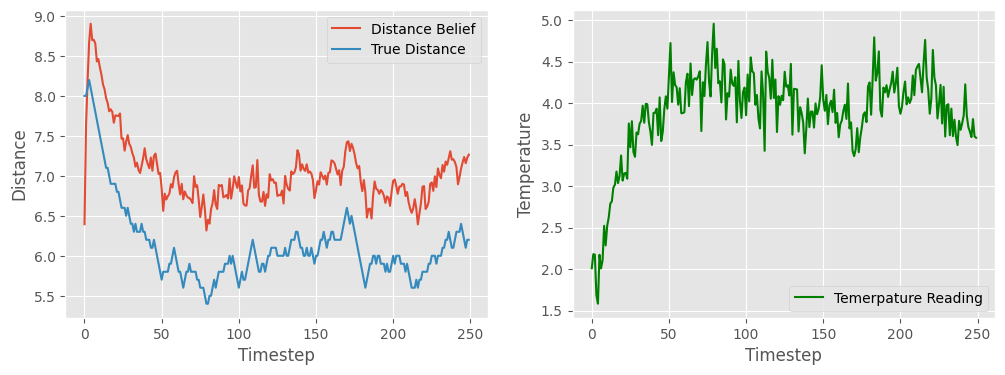
\includegraphics[scale=0.5]{images/pc_example_planning.png}
	\caption{Results of a predictive coding agent equipped with planning using EFE in the Bayesian Thermostat environment. \textbf{Left}: This depicts the difference between the agents belief of its distance to the heat source compared to the true distance it is from the heat source. We observe that the agent is consistently estimating its distance to be greater than the true distance. \textbf{Middle}: This is a plot of the observations (temperature readings) observed by the agent over the episode. We notice that even though the agent did not have an accurate sense of where they were in the environment, they were able to consistently receive preferable observations. This is due to the fact that the dilution of the agent's own distance was offset by a weaker synaptic which in combination meant the agent converged to a reasonable niche within the environment. \textbf{Right}: This is a plot of the variational free energy after inference and learning at each time-step.}
	\label{fig:pc_example_planning}
\end{figure}

\

We observe that the agent consistently receives preferable temperature readings from around 50 time-steps onward and remains in this range until the end of the episode. In this sense, the agent has successfully ``solved'' the environment. What is particularly interesting, however, is the distorted beliefs the agent maintains about its own distance from the heat source. Throughout the episode, there is a distinct discrepancy between the agent's actual position and where it believes it is.

\

The reason the agent is still able to ``solve'' the environment despite this discrepancy lies in the range of synaptic weights, which effectively compensate for the belief distortion. The average weight over the last 200 time-steps is $-0.865$, and its average belief about its distance during the same period is $6.9$. Based on the agent's beliefs about the environment's dynamics, it perceives itself to have solved the environment since $6.9 \times -0.865 + 10 = 4.03$. While this could be avoided by introducing additional components that enforce a more accurate representation of the environment, this result raises two interesting points for discussion.

\

The first, which we have touched on previously, is the difficulty the agent faces in jointly inferring both its location and the dynamics of the environment when there is some degree of error in one or both. The circular relationship between these elements means the agent can end up in a situation where ``two wrongs make a right.'' In other words, errors in the model's dynamics can offset errors in its belief about its position.

\

The second point is related to how we interpret the hidden state $x$. We have been referring to $x$ as the agent's belief about its distance from the heat source. But in reality, it is simply a latent variable that the agent must infer. We have assumed the structure of the environment pushes this variable to align closely with the actual distance. However, if we relaxed certain assumptions or introduced more complex relationships between temperature and distance, this latent variable could represent something entirely different. In such a scenario, our intuition that $x$ represents distance would break down.

\

This leads to an important, more philosophical observation: how we, as humans, represent our environments internally may not correspond directly to the ``true'' states of the world. There is no guarantee that the latent representations we form are consistent across individuals. This is why our communication about the environment is grounded in shared observations, rather than in our internal states. Nevertheless, for the purposes of this report, the hidden state could represent anything, or nothing specific at all. This idea will become clearer in the next section, where we treat the size of the hidden state as a hyper-parameter.


\subsection{Temporal Predictive Coding}

In our discussion thus far we have only considered a single hidden state and single observation dimension. This model was useful for demonstration about the internal dynamics of predictive coding as well as revealing some of the complexities that arise even in simple situations with the model we are considering. We aim now to extend our understanding of predictive coding models to incorporate a deeper hierarchical structure. \citep{friston2008hierarchical} We will then use the slightly more complicated formulation of the generative, and variational components of the model to define the core component for this implementation section - \textit{temporal predictive coding}. This model of predictive coding aims to incorporate the correlation of sensory data into the components of the model. Once again, predictive coding does not include the notion of planning so we will be extending with model using EFE in a very similar way to what we have done in the previous section.

\subsubsection{Hierarchical Predictive Coding}

The success of deep neural networks in machine learning have demonstrated that having hierarchical sets of latent variables is key to enabling methods to learn powerful abstractions and to handle intrinsically hierarchical dynamics of the sort humans intuitively perceive. The predictive coding schemes previously introduced can be straightforwardly extended to handle hierarchical dynamics of arbitrary depth, equivalently to deep neural networks in machine learning.

\

This is done by postulating multiple layers of latent variables, $x_1, \dots, x_L$ and defining the generative model as:

\begin{equation}
	p(x_0, \dots, x_L) = p(x_L) \prod_{l = 0}^{L - 1} p(x_l | x_{l-1})
\end{equation}

Where $x_l | x_{l - 1} \sim N(f_l(x_{l + 1}; \theta_{l + 1}) , \Sigma_l)$ and the final layer $x_L \sim N(\bar{x_L}, \Sigma_L)$ has some arbitrary prior $\bar{x_L}$ and the latent variable at the bottom of the hierarchy is set to what was actually observed $x_0 = y$. 

\

Similarly, we define a variational posterior for the generative model that can be decomposed for each layer:

\begin{equation}
	q(x_{1:L}) = \prod^L_{l = 1} \delta(x_l - \phi_l)
\end{equation}

The variational free energy can thus be written as the sum of prediction errors on each level:

\begin{equation}\label{eq:vfe_pc_hierarchical}
\mathcal{F} = \prod_{l = l}^{L} \Sigma_l^{-1} \epsilon_l^2 + \ln 2 \pi \Sigma_l
\end{equation}

Where $\epsilon_l = \phi_l - f_l(\phi_{l + 1}; \theta_{l + 1})$\footnote{Which is subtly different to the error in the previous section. This is simply notional, and is due to the difference between $\Sigma$ being the co-variance matrix while $\sigma$ is standard deviation.}

\

Since the free energy can be nicely divided into sum of layer-wise prediction errors, it is natural to express the dynamics of $\phi$ and $\theta$ in a similar way:

\begin{equation}
	\begin{aligned}
		\frac{d\phi_l}{dt} &= - \frac{\partial \mathcal{F}}{d\phi_l} = \Sigma_{l - 1}^{- 1} \epsilon_{l - 1} \frac{\partial f_{l - 1}(\phi_{l}; \theta_{l})}{\partial \phi_{l}} - \Sigma_{l}^{-1} \epsilon_l \\
		\frac{d\theta_l}{dt} &= - \frac{\partial \mathcal{F}}{d\theta_l} = \Sigma_{l - 1}^{- 1} \epsilon_{l - 1} \frac{\partial f_{l - 1}(\phi_{l}; \theta_{l})}{\partial \theta_{l}}
	\end{aligned}
\end{equation}

\subsubsection{Temporal Predictive Coding}

In our examples and models of predictive coding we have mostly been focussed on treated each sensory observation independently. The problem with this approach is that sensory observations are highly correlated through time. So an essential feature of any model of the brain is how the model is able to handle this dynamically changing and correlated data. We aim to demonstrate this through a predictive coding model called temporal predictive coding (tPC). 

\

The generative structure of the temporal predictive coding model is a hidden Markov model (HMM). This means that for every time-step $t$ there exists an observation $y_t$ that only depends on the underlying hidden state at that point in time, $x_t$. The hidden state only depends on the previous hidden state $x_{t-1}$. While this is the usually structure of a HMM, \citet{millidge2024temporal} compared the models performing to Kalman filter in a Bayesian filtering task, which required an additional control unit, $u_t$, which too effects the underlying state. See Figure \ref{fig:hmm} for the probabilistic graphical model of the described HMM. 

\

\begin{figure}[h]
    \centering
    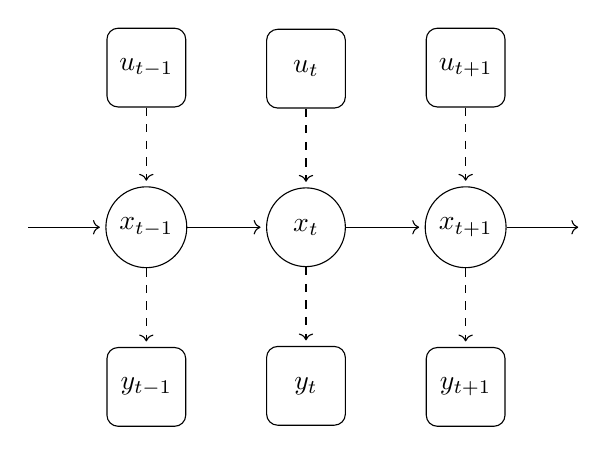
\begin{tikzpicture}[
        every node/.style={circle, draw, minimum size=1cm, node distance=1cm},
        state/.style={rectangle, rounded corners, draw, minimum size=1cm, node distance=1cm},
        ->, 
        shorten >=2pt, 
        auto
    ]

    % Hidden states
    \node (x1) at (0, 0) {$x_{t-1}$};
    \node (x2) [right=of x1] {$x_t$};
    \node (x3) [right=of x2] {$x_{t+1}$};

    % Controls
    \node[state] (u1) [above=of x1] {$u_{t-1}$};
    \node[state] (u2) [above=of x2] {$u_{t}$};
    \node[state] (u3) [above=of x3] {$u_{t+1}$};

    % Observations
    \node[state] (y1) [below=of x1] {$y_{t-1}$};
    \node[state] (y2) [below=of x2] {$y_{t}$};
    \node[state] (y3) [below=of x3] {$y_{t+1}$};

    % Transitions between hidden states
    \draw[->] (x1) to (x2);
    \draw[->] (x2) to (x3);
    
    % Actions
    \draw[->, dashed] (u1) -- (x1);
    \draw[->, dashed] (u2) -- (x2);
    \draw[->, dashed] (u3) -- (x3);
    
    % Emissions
    \draw[->, dashed] (x1) -- (y1);
    \draw[->, dashed] (x2) -- (y2);
    \draw[->, dashed] (x3) -- (y3);

    % Arrow from the left to x1
    \draw[->] ($(x1)+(-1.5, 0)$) -- (x1);

    % Arrow from x3 to the right
    \draw[->] (x3) -- ($(x3)+(1.5, 0)$);

    \end{tikzpicture}
    \caption{A Hidden Markov Model representation of the temporal predictive coding model (tPC). The model represents the recurrent connection between hidden states in the previous time step. The translations between hidden states are done by an activation on the previous level of activity, in this case this activation was a sigmoid function. The `transition' matrix A is then applied to these activated values, further the effect of a control input $u_t$ is applied to the value of each hidden state by a multiplication with the `control' matrix. The value of the hidden state is assumed to then generate the observations $y_t$. This emission is similarly done by passing hidden states through the activation function, with a weight matrix then applied to the output. Additionally, the emission component is equipped with a bias term in the model to scale the output to better represent the observations within the environment.}
    \label{fig:hmm}
\end{figure}

This model handles the correlation between sensory data by introducing the recurrent connection between hidden states. Machine learning and statistics have many established models with this recurrent connection established. Which include recurrent neural networks (RNN), and more advanced versions of RNN's like  Long Short-Term Memory (LSTM) models. However, for training these models use a method called backpropagation through time (BPTT). BPTT is considered to be biologically implausible because the brain processes inputs sequentially and in real time, and does not appear to have the ability to unfold sequences of computation through time. \citep{millidge2024temporal}

\

From the graphical model of the HMM we can write out specific equations for the dynamics of the states and observations in what is called the state-space representation:

\begin{equation}\label{eq:tpc}
	\begin{aligned}
		x_t &= A f(x_{t-1}) + B u_y + \omega_x \\
		y_t &= C f(x_t) + \omega_y
	\end{aligned}
\end{equation}

The $A$ matrix which we will call the `transition' matrix - encodes how the hidden states are expected to change from one time-step to the next. The $B$  encodes the effect of actions $u$ on the hidden states, which is called the `control' matrix. Finally the $C$ is the `emission' matrix translating the underlying state to observations\footnote{This is not the preference over observations that is traditionally also defined using `C' in active inference.}. While $\omega_x, \omega_y$ are Gaussian noise. We can now translate this state-space representation into our tPC generative model:

\begin{equation}
\begin{aligned}
	x_t | x_{t-1}, u_{t} &\sim N( A f(x_{t-1} + B u_{t}), \Sigma_x) \\
	y_t | x_t &\sim N( C f(x_t) + c, \Sigma_y)
\end{aligned}
\end{equation}

The structure of this generative model closely mirrors a typical state-space representation. The key addition is a bias term, $c$, in the emission model. This term was not included in the original formulation by \citet{millidge2024temporal}, where the model was used exclusively for filtering tasks. In those cases, scaling the output was unnecessary. However, since we are applying this model to a control task, it becomes essential to scale the predicted output to minimise the prediction error. As discussed in the previous section, minimising prediction error is closely tied to minimising variational free energy, which remains our ultimate goal with each observation.

\

It is important to note that a bias term is not required in the temporal transition component of the model. This is because the hidden states in our model do not need to represent physical quantities directly. Instead, they are free to evolve in a way that is internally consistent within the model. As such, there is no need to scale them to fit external data, allowing them to serve purely as latent variables that facilitate the model's performance.

\

The second key component of the model is the activation function, $f$. In this case, we have chosen the sigmoid function. While the sigmoid does not have strong biological roots, other similar functions, such as the softmax, exhibit greater biophysical plausibility. Specifically, functions like the softmax reflect the dynamics of spiking neuron populations, where synaptic input is converted into neuronal firing rates in a manner consistent with observed biological processes \citep{deco2008brain}.

\

We will be assuming the Dirac-delta distribution as our variational posterior distribution, $q= \delta(x - \phi)$. We can then define the variational free energy objective:

\begin{equation}
    \begin{aligned}
        \mathcal{F} &= \frac{1}{2} \left(y_t - C f\left(x_t\right) - c\right)^T \Sigma_y^{-1} \left(y_t - C f\left(x_t\right) - c\right) \\
        &\quad + \frac{1}{2} \left(x_t - A f\left(\hat{x}_{t-1}\right) - B u_t\right)^T \Sigma_x^{-1} \left(x_t - A f\left(\hat{x}_{t-1}\right) - B u_t\right)
    \end{aligned}
\end{equation}

Still equipped with the assumption that the components of the model change over time to minimise the variational free energy. We are able to take the partial derivative of the free energy function to define our update equations:

\begin{equation}\label{eq:tpc_neural}
	-\frac{\partial \mathcal{F}}{\partial\phi_k}=-\epsilon_x+f^{\prime}\left(\phi_k\right) \odot C^T \epsilon_y
\end{equation}

We again note the temporal dynamics here. In the inference process we will be taking multiple gradient descent steps with respect to the posterior variational parameters. So, once $\phi$ has converged we will denote this as $\phi_K$. In which case the update is: $x_t = \phi_K$. We can take the partial derivative with respect to the other variables of interest:

\begin{equation}
    \begin{aligned}
        \Delta A &= -\eta \frac{\partial \mathcal{F}}{\partial A} = \eta \epsilon_x f\left(\hat{x}_{t-1}\right)^T \\
        \Delta B &= -\eta \frac{\partial \mathcal{F}}{\partial B} = \eta \epsilon_x u_t^T \\
        \Delta C &= -\eta \frac{\partial \mathcal{F}}{\partial C} = \eta \epsilon_y f\left(x_t\right)^T \\
        \Delta c &= -\eta \frac{\partial \mathcal{F}}{\partial c} = \eta \epsilon_y
    \end{aligned}
\end{equation}

Where $\epsilon_x := \Sigma_x^{-1}(x_t - A f(\hat{x}_{t-1}) - Bu_t)$ and $\epsilon_y := \Sigma_y^{-1}(y_t - C f(x_t) - c)$

\

These updates correspond to the (M) step in the EM scheme. We will again constrain the updates of our components by a learning rate, $\eta$, the dynamics of this hyper-parameters will be discussed later in this section. What is also to note is that $\hat{x_{t-1}}$ denotes the predicted hidden state in the previous time-step, while $x_t$ denotes the relaxed neural activity from the (E) step in \refp{eq:tpc_neural}. 

\subsubsection{Extending to Planning}

The extension to planning will happen in exactly the same fashion as the previous model. Meaning we will only be considering a policy of length one which means the model is only inferring what next action to perform. And similarly, we will be EFE with respect to each action and passing the negated value through the softmax function to create a distribution over actions that we then sample from to determine the next action. 

\

The departure from the previous model is that the agent is also tasked with learning the effects of its actions on the environment. This is represented in the model through the $B$ matix. The expected next state is then expressed as:

\begin{equation}
	x_{t+1} | u_t \sim N(A f(\hat{x}_{t}) + B u_{t}, \Sigma_x)
\end{equation}

We will then use the mean of this distribution, $\mu_{t+1} := A f(\hat{x}_{t}) + B u_{t}$ to create the distribution over observation in the next time-step:

\begin{equation}
	y_{t+1} | u_t \sim N( C f(\mu_{t+1}) + c, \Sigma_y)
\end{equation}

\subsubsection{Partially Observable Cart-Pole}

\begin{figure}[htbp]
    \centering
    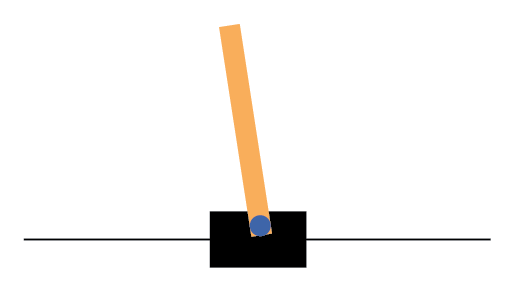
\includegraphics[scale=1.5]{images/cart_pole.png}
    \caption{A sample image from the OpenAI cart-pole environment}
    \label{fig:cart_pole}
\end{figure}

The cart-pole is a well-known environment used in reinforcement learning baselines. It requires controlling a cart with a pole attached, with the goal of balancing the pole upright. The environment typically provides observations such as the position and velocity of the cart, as well as the angle and angular velocity of the pole. However, since velocity naturally includes some temporal information, which our model is specifically designed to capture, we modified the OpenAI \citep{towers2024gymnasium} environment to reduce the observations to velocity only.

\

Furthermore, while the default environment assigns a reward at each time step, we redefined the objective to focus on maintaining the pole upright and the cart centred on the screen, similar to the approach taken by \citet{millidge2019combining}. This modification fundamentally changes the control problem, as the reward feedback is now much denser. Nonetheless, this variation presents a significantly greater challenge to the predictive coding model compared to previous environment.

\subsubsection{Results and Discussion}

\begin{figure}[htbp]
    \centering
    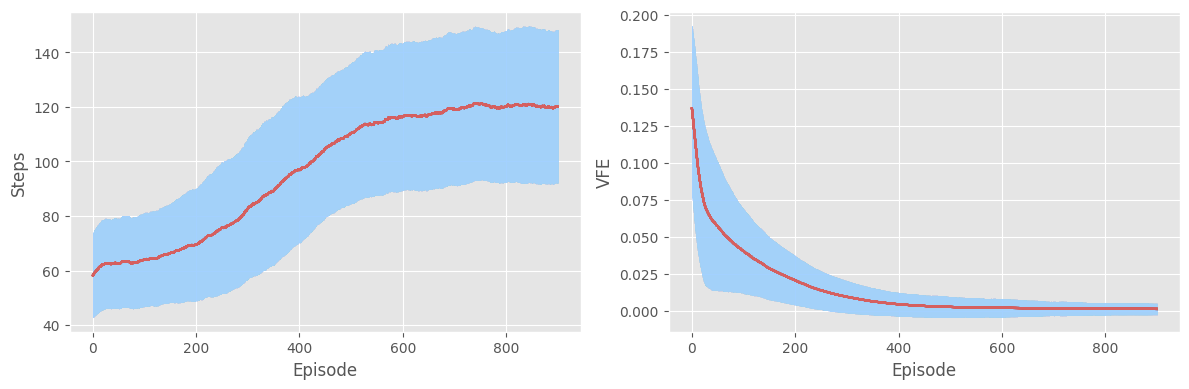
\includegraphics[scale=0.5]{images/tpc.png}
    \caption{Results of from the partially observable cart pole environment using temporal predictive coding with planning using expected free energy. \textbf{Left}: These are the averaged smoothed episodes steps across runs. The experiment used 25 runs with each one consisting of 1000 episodes, each of these runs were then smoothed using a 100 episode moving average, these moving averages themselves were then averaged together to give the red line. The blue area depicts a confidence interval for this average. This represents a single standard deviation from the average moving average. \textbf{Right}: This depicts the associated variational free energy to the left plot. Meaning that this depicts the red line depicts the average moving average of this variational free energy per episode. The VFE per episode consisted of averaging the free energy per observation. The blue area similarly depicts a single standard deviation from the mean.}
    \label{fig:tpc_results}
\end{figure}

The experiment involved 1000 episodes across 25 separate runs, with the results are shown in Figure \refp{fig:tpc_results}. he plot on the left, which illustrates the number of time steps the agent was able to balance the pole, demonstrates significant improvement after around 250 episodes, with the agent eventually maintaining balance for over 120 time steps. This indicates a non-trivial level of learning in this task. For reference, a simple baseline control rule—where the agent moves left if the pole leans—achieves an average of 50 time steps \citep{millidge2019combining}. Additionally, a clear correlation is observable between the average variational free energy (VFE), depicted on the right, and task performance. When the model successfully reduces VFE, performance improves. Interestingly, once VFE converges near zero, performance also plateaus.

\

The variance in the tPC model's balance performance remains noisy, however. In some runs, the agent successfully balanced the pole for up to 500 time steps (the maximum), while in others, it dropped back to around 50 time steps. To address this, we applied exponential decay to the learning rate parameter $\eta$. While this adjustment helped the agent achieve better average performance across episodes, it did not significantly reduce the episode-to-episode variance.
\

A natural question arises: how well is the agent learning the dynamics of the environment? VFE provides some insight, as it acts as an upper bound on the agent's surprise given the observation, but prediction error offers a more precise measure. If the agent is in a particular state and selects an action, part of its decision-making process involves projecting itself one step into the future—a process discussed in the previous section. We can therefore compare the accuracy of these predictions by calculating the norm of the predicted observation (from the counterfactual process in the expected free energy calculation) against the actual observation. These results, shown in Figure \ref{fig:tpc_pred_error}, reveal that prediction errors are closely correlated with VFE, as expected. However, the model does not converge to zero prediction error, indicating it cannot fully model the environment’s dynamics.

\

This result is not unexpected. The cart-pole environment’s dynamics are governed by a second-order system \citep{florian2005CorrectEF}, which poses a challenge for a single-layer network, even with a non-linear activation function.

\begin{figure}[htbp]
    \centering
        \begin{minipage}[c]{0.6\textwidth}
        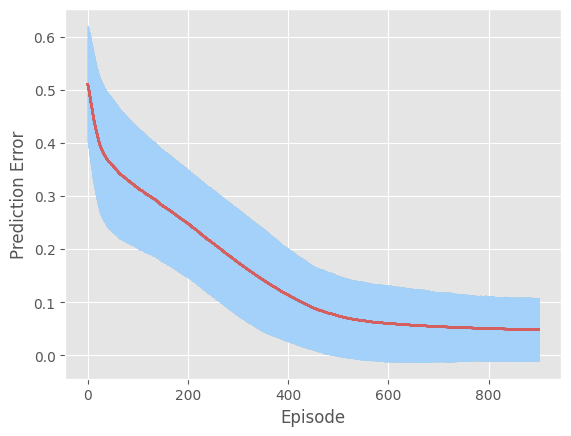
\includegraphics[width=\textwidth]{images/pred_error.png}
    \end{minipage}
    \hfill
    \begin{minipage}[c]{0.35\textwidth}
        \caption{The averaged moving average plot for the prediction errors in the experiment. The red line depicts the average moving average from the 25 runs across episodes, while the blue shaded region depicts a single standard deviation confidence interval.}
        \label{fig:tpc_pred_error}
    \end{minipage}
\end{figure}

\

As mentioned in the previous section, we cannot directly compare the results of this experiment with other cart-pole algorithms, as the objective used in this model involves a far denser reward space. Nonetheless, \citet{millidge2024temporal} similarly used observations from the environment to define the preference distribution for their active inference agent. Their model, which employed a hierarchical predictive coding framework in a fully observable version of Cart-Pole, achieved an average of slightly less than 100 time steps across 50 trials.

\

A key factor in the performance of this model is its sensitivity to initial conditions, particularly the weight initialisation in the various matrices. In some instances, poor weight initialisation resulted in no learning across the 1000 episodes, with the agent balancing the pole for an average of only 9 time steps. To address this issue, we fixed the randomisation seed for weight initialisation across all runs in our experiments. It is important to note that this sensitivity to initialisation is not unique to this model and does not indicate an inability to scale to more complex tasks. Even deep neural networks suffer from similar weight initialisation challenges \citep{mishkin2016needgoodinit}.

\ 

The dimension of the latent space also enters into the model as a hyperparameter. The hidden state in this model as not necessarily aiming to represent anything specific about the environment. We observed the best performance for our model with a dimension of between $6$ and $8$. 

\subsection{Message Passing}

Predictive coding is often presented as a neural process theory, offering a mechanistic explanation of cognitive functions and their neuronal underpinnings. However, when constructing active inference models, predictive coding can also be understood as a variational inference algorithm for performing approximate Bayesian inference. Predictive coding is not unique in this role - many statistical inference algorithms have been suggested to have neurobiological relevance, one of which is \textit{message passing}.

\

In this report, we will review and implement a specific message passing algorithm called \textit{belief propagation}. Belief propagation allows for the exact computation of marginal posteriors, though this precision comes at the cost of greater architectural complexity compared to simpler algorithms such as variational message passing. Our focus will be on message passing over Forney-style factor graphs (FFG), also known as normal factor graphs. These graphs provide a clear graphical representation of the relationships between variables and factors within a joint probability distribution. By expressing a joint probability distribution in the form of an FFG, we can derive messages passed between nodes on the graph, enabling efficient and exact Bayesian inference—provided that the graph has no loops.


\subsubsection{Forney-style Factor Graphs and Belief Propagation}

A Forney-style factor graph (FFG) is a graphical representation of a factorised probabilistic model, where edges represent variables and nodes specify relations between them. The purpose of expressing a joint probability distribution as an FFG is to highlight dependencies between variables, facilitating more efficient inference. To illustrate this, consider a joint probability distribution of the form:

\begin{equation}\label{eq:ffg_inference_example}
	p(x_1, x_2, x_3) = \frac{1}{Z}f_a(x_1)f_b(x_1, x_2)f_c(x_2, x_3)
\end{equation}

\begin{figure}[h]
    \centering
	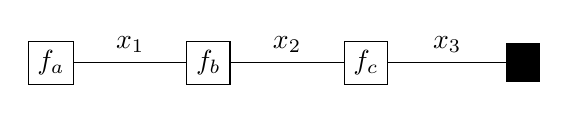
\begin{tikzpicture}[node distance=2cm, auto, ->, >=]

    	% Define nodes
	    \node (fa) [draw, rectangle] {$f_a$};
    	\node (fb) [draw, rectangle, right of=fa] {$f_b$};
	    \node (fc) [draw, rectangle, right of=fb] {$f_c$};
	    \node (d) [draw, rectangle, right of=fc, fill=black] {$d$};

	    % Draw arrows
    	\draw[->] (fa) -- node {$x_1$} (fb);
	    \draw[->] (fb) -- node {$x_2$} (fc);
    	\draw[->] (fc) -- node {$x_3$} (d);

	\end{tikzpicture}
	\caption{FFG for the joint probability distribution in \refp{eq:ffg_inference_example}. Each factor is displayed in block, with each variable represented as an edge in the graph. The observed variable is depicted as a black node, this represents the $\delta$ function to clamp the value of the variable $x_3$.}
	\label{fig:belief_propogation}
\end{figure}

Where $Z$ is a normalisation constant. Then let us consider the problem of inferring the marginal distribution of $x_2$ given some observation of $x_3$.

\begin{equation}
\begin{aligned}
	p(x_2 | x_3 = \widehat{x_3}) &\propto \int_{x_1, x_3} p(x_1, x_2, x_3) \delta(x_3 - \widehat{x_3}) \ dx_2 dx_3 \\
	&\propto \int_{x_1, x_3} f_a(x_1)f_b(x_1, x_2)f_c(x_2, x_3) \delta(x_3 - \widehat{x_3}) \ dx_2 dx_3
\end{aligned}
\end{equation}

We use the Dirac function, $\delta$, to clamp the variable to take the observed value. 

\

The key point is that not all factors (functions) depend on every variable, which enables us to 'push in' the integrals. This lets us express the posterior in terms of more easily computable components, or \textit{messages}.

\begin{equation}
\begin{aligned}
	p(x_2 | x_3 = \widehat{x_3}) &\propto \int_{x_1, x_3} f_a(x_1)f_b(x_1, x_2)f_c(x_2, x_3) \delta(x_3 - \widehat{x_3}) \ dx_1 dx_3 \\
	&\propto \overbrace{\int_{x_1}f_a(x_1)f_b(x_1, x_2)}^{\mu_{f_a \to x_2}} \ dx_1 \underbrace{\int_{x_3}f_c(x_2, x_3) \overbrace{\delta(x_3 - \widehat{x_3})}^{\mu_{x_3 \to f_c (x_3)}} \ dx_3}_{\mu_{f_c \to x_2}} \\
	&\propto \mu_{f_b \to x_2} \mu_{f_c \to x_2}
\end{aligned}
\end{equation}

$\mu$ is what we call a message. In the FFG we will be exploring the factors, $f$, will also be probability distributions. This means that these messages can just be considered as unnormalised probability distributions - otherwise known as beliefs. Passing these messages around the factor graph is what gives rise to the notion of belief propagation.


\paragraph{Remark} The point that has not yet been address is the normalisation of these messages in order to form a valid probability distribution. This normalisation only requires the evaluation of low-dimensional integrals over local variables which makes it a more tractable computation. What is more, if all messages are Gaussian and any other node function is linear. The integrable has a closed form. \citep{bagaev2021reactive}

\paragraph{Relation to Free Energy} As we have discussed in pervious sections, the Bayesian posterior is optimal with respect the variational free energy and therefore surprise. What is interesting to note is that belief propagation and variational message passing \citep{winn2005variational} can both be framed as VFE minimisation augmented with the Bethe factorisation assumption. \citep{yedida2005constructing} Which gives message passing algorithms that can incorporate both the computational benefits of variational message passing and belief propagation. \citep{bagaev2021reactive} 

\paragraph{Equality Factor} Within a FFG we depict a variable as an edge connecting two factors. As opposed to a bipartite graph where they are depicted as nodes with edges corresponding to the relationship between variables and factors. This introduces a constraint that a variable can only be a function of two factors. We resolve this constraint by an equality factor. The equality factor resolves this situation by constraining the information about three variables to be equal. 	\citep{cox2019factor} More precisely:

\begin{equation}\label{eq:equality_factor}
	f_{=}(x, y, z) = \delta(x - z)\delta(x - y)
\end{equation}

Meaning that:

\begin{figure}[h]
    \centering
    \begin{minipage}{0.45\textwidth}
        \begin{equation*}
        \begin{aligned}
        	\mu_{\circled{3}}(z) &= \int \int \mu_{\circled{1}}(z) \mu_{\circled{2}}(z) \, dx_1 \, dx_2 \\
        	&= \mu_{\circled{1}}(z) \mu_{\circled{2}}(z)
        \end{aligned}
        \end{equation*}
    \end{minipage}
    \begin{minipage}{0.45\textwidth}
        \centering
        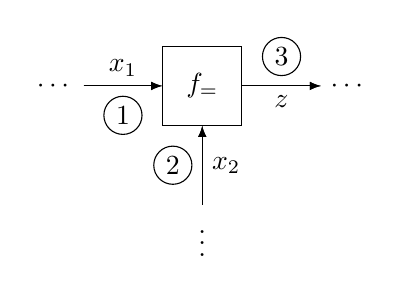
\begin{tikzpicture}[auto, node distance=1cm, >=latex]

            % Nodes
            \node (ldots) {$\cdots$};
            \node [right=of ldots] (equal) [draw, minimum size=1cm] {$f_=$};
            \node [right=of equal] (rdots) {$\cdots$}; % Three dots
            \node [below=of equal] (bdots) {$\vdots$};

            % Arrows and edge labels
            \draw[->] (ldots) -- node[above]{$x_1$}(equal);
            \draw[->] (ldots) -- node[below]{\circled{1}}(equal);

            \draw[->] (bdots) -- node[right]{$x_2$}(equal);
            \draw[->] (bdots) -- node[left]{\circled{2}}(equal);

            \draw[->] (equal) -- node[below]{$z$}(rdots);
            \draw[->] (equal) -- node[above]{\circled{3}}(rdots);

        \end{tikzpicture}
        \label{fig:equality_factor}
    \end{minipage}
    \caption{Example of the message passing behaviour over an equality factor}
\end{figure}

\subsubsection{Mountain Car}

The mountain car environment describes an environment where a car is in a valley, and the car is not powerful enough to reach its target on the side of the mountain - higher up than it currently is. Thus the car is required to move backwards and generate enough force to then move to its target on the other side of the valley. 

\begin{figure}[htbp]
    \centering
    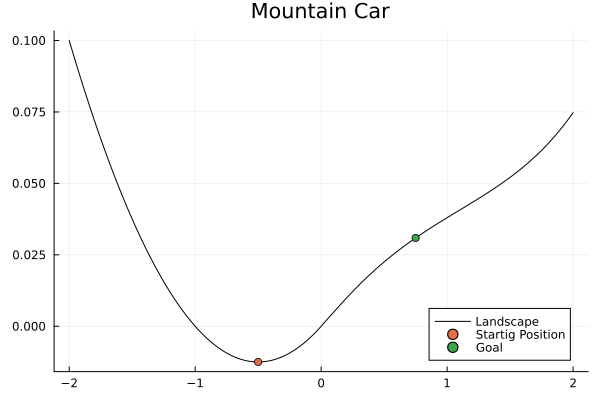
\includegraphics[scale=0.5]{images/mountain_car_plot.png}
    \caption{The landscape of the mountain car environment. Including the starting and target position for the model.}
    \label{fig:markov_blanket}
\end{figure}

\

This environment was originally proposed by \citet{moore90efficientmemory}, however the specific physics that are being used are based on the environment used in \citet{ueltzhoffer2018deep, van2019simulating}. Specifically, let us define the environmental states $z_t = (\phi_t, \dot{\phi}_t)$ depending on the position ($\phi_t$) and velocity of the car ($\dot{\phi}_t$). The environment is fully observable, meaning that the observations generated, $y_y$ , will be a reflection of these underlying states. The evolution of the state can then be described as:

\begin{equation}
	\begin{aligned}
		\dot{\phi}_t &= \dot{\phi}_{t-1} + F_g(\dot{\phi}_{t-1}) + F_f(\dot{\phi}_{t-1}) + F_a(a_t) \\
		\phi_t &= \phi_{t-1} + \dot{\phi}_t
	\end{aligned}
\end{equation}

Where $F_g$ is the gravitational force of the hill landscape that depends on the car's positions:

\begin{equation}
F_g(\phi) = \left\{
	\begin{aligned}
		&- 0.05 (2 \phi + 1), \ & \text{for } \phi < 0 \\
		&- 0.05 \left[ (1 + 5\phi^2 )^{-\frac{1}{2}} + \phi^2( 1 + 5\phi^2)^{-\frac{3}{2}} + \frac{1}{16} \phi^4\right] & \text{otherwise}
	\end{aligned}
	\right.
\end{equation}

$F_f$ is the friction of the car are is defined as $F_f(\dot{\phi}) = -0.1 \dot{\phi}$ and $F_a(a)$ is the engine force $F_a(a) = 0.04 \tanh(a)$ which restricts the force exerted by the car to be between -0.04 ad 0.04.

\subsubsection{Model}

Let us now define the form of the generative model. This model is derived from \citet{van2019simulating}, with some adjustment which will be highlighted. By using the Markov property of the environment we can define our generative model:

\begin{equation}\label{eq:mountain_car_generative_model}
	p_t(x, y, u) \propto p(x_{t-1}) \prod_{k=t}^{t + T} p(y_k | x_k) p(x_k | x_{k-1}, u_k)p(u_k)\tilde{p}(y_k)
\end{equation}

The Forney-factor graph for this generative model can be seen in Figure \ref{fig:online_ai_ffg}. The precise distributions defined for each component as:

\begin{equation}
\begin{aligned}
	p(y_k | x_k) &= N(x_k, \ \Sigma_y ) \\
	p(x_k | x_{k-1}, u_k) &= N(h(u_k) + g(x_{k-1}), \ \Sigma_x) \\
	p(u_k) &= N(0, \ \Sigma_u)
\end{aligned}	
\end{equation}

The component we have neglected to mention above is the preference distribution. The model initialises the preference distribution as vague for the first $T$ time-steps. After which it is restricted to a concentrated distribution around the goal observation:

\begin{equation}
	\tilde{p}(y_k) = \left\{
	\begin{aligned}
		& N\left((0, 0), \ 10^{4} \times \mathbb{I}_2 \right) , \ & \text{for} \ k < T \\
		& N\left((0.75, 0), \ 10^{-4} \times \mathbb{I}_2 \right) , \ & \text{otherwise}
	\end{aligned}
	\right.
\end{equation}

The algorithm for each time-step using this model can be summarised as comprising of three distinct steps:

\paragraph{1. Act-Execute-Observce} - We first select the \textbf{mean} of the marginal distribution over the controls, $u_k$. We then execute this actions on the environment and observe the new observations generated from the environment, $y_k$.

\paragraph{2. Infer} - Having executed a new action and generated a new observation at time $k$ we will then clamp these within the generative model and perform message passing to infer the posterior distribution of the generative model. This is the step where we require belief propagation.  

\paragraph{3. Slide} - In this step we instantiate the generative model by specifying the new prior to time $t+1$ as well sliding the inference horizon $T$. Specifically:

More specifically:


\begin{equation}
\begin{aligned}
    p_{t+1}(x, y, u) \propto 
    &\underbrace{\int \overbrace{p\left(x_{t-1}\right) p\left(x_t | x_{t-1}, u_t\right) p\left(y_t | x_t\right)}^{\text{first slice}} 
    \overbrace{\delta\left(u_t - \widehat{u_t}\right) \delta\left(y_t - \widehat{y_t}\right)}^{\text{action and observation}} dx_{t-1} du_t dy_t}_{\text{new prior - } p(x_t)} \\
    &\underbrace{\left(\prod_{k=t+1}^{t+T} p\left(x_k | x_k\right) p\left(x_k | x_{k-1}, u_k \right) p\left(u_k\right) \tilde{p}\left(y_k\right)\right)}_{\text{unaltered mid-section slices}} \\
    &\underbrace{p\left(y_{t+T+1} | x_{t+T+1}\right) p\left(x_{t+T+1} | x_{t+T}, u_{t+T+1}\right) p\left(u_{t+T+1}\right) \tilde{p}\left(y_{t+T+1}\right)}_{\text {add slice at horizon }}
\end{aligned}
\end{equation}

Upon inspection we can see that the new prior is nothing but the message coming from the equality node in Figure \ref{fig:online_ai_ffg}. 

\paragraph{Non-Linearity} The physical dynamics of the environment are not linear as described in the previous section. The issue with these non-linearities is that incoming messages from an exponential family of distributions is not guaranteed to be part of the exponential family when output. \citep{van2019simulating} Thus, we will perform a linear approximation of the change in hidden states over time as given by $F_g$ and $F_f$, this function is denoted as $g$. As well as a linear approximation of the control $F_a$ which is denoted $h$. The exact approximation technique was derived specifically for non-linearities in factor graphs \citep{petersen2018approximate}. 

\begin{figure}[h]
    \centering
\begin{tikzpicture}[auto, node distance=0.75cm, >=latex]

    % Nodes
    \node (dots) {$\cdots$}; % Three dots
    \node [right=of dots] (g) [draw, minimum size=1cm] {$g$};
    \node [right=of g] (plus) [draw, minimum size=1cm] {$+$};
    \node [right=of plus] (N) [draw, minimum size=1cm] {$p(x_k | x_{k-1}, u_k)s$};
    \node [right=of N] (equal) [draw, minimum size=1cm] {$=$};
    \node [right=of equal](dots1) {$\cdots$}; % Three dots

    \node [above=of plus] (h) [draw, minimum size=1cm] {$h$};
    \node [above=of h] (uk) [draw, minimum size=1cm] {$p(u_k)$};
    
    \node [below=of equal] (yk) [draw, minimum size=1cm] {$p(y_k | x_k)$};
    \node [below=of yk] (tilde_yk) [draw, minimum size=1cm] {$\tilde{p}(y_k)$};

    % Arrows and edge labels
    \draw[->] (dots) -- node[above] {$x_{k-1}$} (g);
    \draw[->] (g) -- (plus);
    \draw[->] (h) -- (plus);
    \draw[->] (uk) -- node[right]{$u_{k}$}(h);
    \draw[->] (plus) -- (N);
    \draw[->] (N) -- (equal);
    \draw[->] (equal) -- node[above]{$x_k$}(dots1);

    \draw[->] (equal) -- (yk);
    \draw[->] (yk) -- node[right]{$y_k$}(tilde_yk);

\end{tikzpicture}
\caption{A Forney-factor Graph for the generative model used in the mountain car environment. Each component will be repeated for each time along the time horizon $T$. The factors within the graph that denote the probability distributions have their arguments included in label. This is redundant since the edges dictate the arguments. This was done for clear reference to the generative model in \refp{eq:mountain_car_generative_model}.}
\label{fig:online_ai_ffg}
\end{figure}

\subsubsection{Results and Discussion}

All results in this environment were computed using the a package for Bayesian inference using message passing called RxInfer.jl \citep{bagaev2023rxinfer}. 

\

\begin{figure}[htbp]
    \centering
    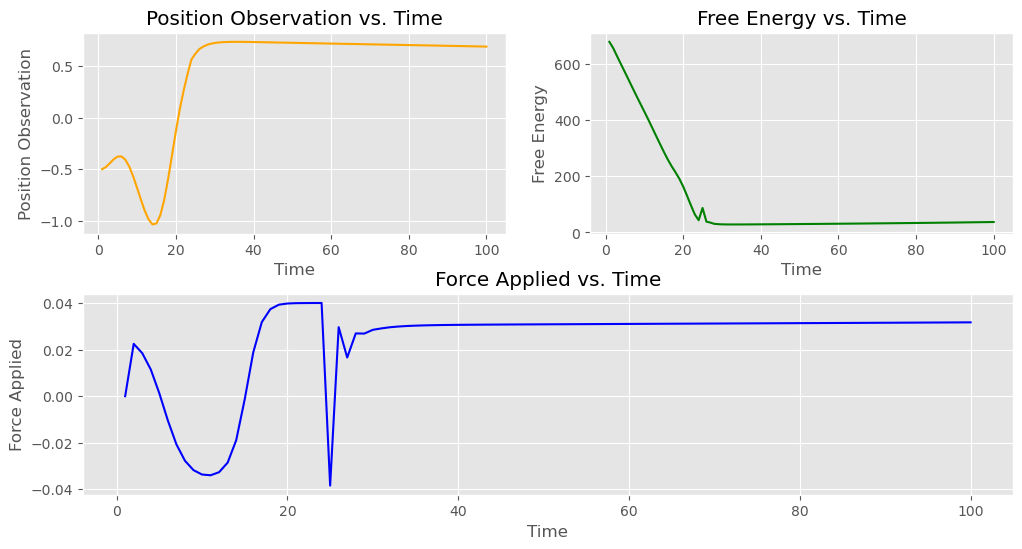
\includegraphics[scale=0.5]{images/mountain_car_results.png}
    \caption{Results from 100 time steps of the active inference agent experiment in the Mountain Car Environment. \textbf{Left}: This is a plot of the observations over the 100 time-steps. We see that the agent is able to reach the goal of a height of 0.75. \textbf{Right}: This is a plot of the Free Energy of each observation over the duration of the episode. \textbf{Bottom}: This is a plot of the force exerted by the agent over the course of the experiment. We observe that indeed the agent is able to move backwards to gain enough potential energy to reach its target height.}
    \label{fig:mountain_car_results}
\end{figure}

The results depicted in Figure \ref{fig:mountain_car_results} show that the active inference agent successfully reached its target height of 0.75 in the Mountain Car environment. To solve this challenge, the agent had to first move backward to gain enough potential energy, then use its forward momentum to climb high enough on the other side of the valley. This is evident in the force-over-time plot. Notably, the agent demonstrates awareness that gradually approaching the goal is not sufficient, and intelligently applies full forward force, followed by full backward force in a braking-like manoeuvre—a highly adaptive behaviour within this environment.

\

Some degree of exploration is clearly necessary within the environment. If the agent behaves greedily, applying full force directly towards the target, it fails to solve the problem. This is a limitation of the current model. By adjusting the variance of the preference distribution $\tilde{p}$ over time, we explicitly induce exploratory behaviour. In fact, if the agent is set with a strict preference distribution for the entire episode, it acts purely greedily and fails to solve the problem.

\

In theory, active inference provides an implicit solution to the exploration vs. exploitation dilemma. However, the current model does not compute actions based on the expected free energy (EFE) of each action; instead, actions are sampled from the mean of the marginal distribution. Modifying the model to incorporate this implicit exploration-exploitation tradeoff would be an intriguing direction for further research.

\clearpage

\section{Conclusion}

In this report, we introduced active inference from two distinct conceptual foundations: what we have referred to as the ``low road'' and ``high road'' to active inference. This distinction was made to highlight that active inference, as a broad and far-reaching framework, can be challenging to approach from a single perspective. By splitting the discussion, we aimed to show that there are multiple ways to begin thinking about and implementing active inference. The framework can be approached from the broad perspective of a persistent biological system, or from a more focused, lower-level view grounded in theories of inference within the brain. Although these approaches differ in their assumptions and fields of application, they can ultimately be seen as performing the same core process of active inference.

\

While understanding the conceptual foundations of active inference is crucial, it is equally important to put the theory into practice by implementing some of the core principles of active inference into models that can solve control and planning problems. We demonstrated that a simple predictive coding generative model of perception, learning, and planning was able to solve a control task in the form of the adaptive Bayesian thermostat. In this environment, the agent successfully inferred its distance from a heat source by observing noisy temperature readings and planned actions by leveraging Expected Free Energy (EFE) to achieve its preferred temperature. Similarly, we showed that a temporal predictive coding model, which accounts for correlations in observations over time, could solve the classic CartPole balancing task. By predicting future states based on past observations, the model was able to plan and execute actions that maintained the pole's balance.

\

Additionally, we demonstrated the effectiveness of belief propagation on a factor graph in the Mountain Car environment. Using biologically plausible message-passing algorithms, the agent successfully planned and executed actions to reverse the car and build enough potential energy to reach the goal state at the top of the mountain. This was achieved by propagating beliefs about the state of the environment and the agent's actions through time, thereby solving a classic control problem in a biologically-inspired way.

\

Though the problems we tackled are relatively simple and there are faster, more efficient algorithms for solving them, the point of these applications was not computational efficiency. Rather, the purpose was to show that we can apply grounded, mathematically rigorous theories like active inference to solve these problems using biologically plausible models. These models, despite their simplicity, illustrate the power and versatility of active inference as a framework for perception, learning, and action in uncertain environments.

\newpage

\bibliography{references}
\addcontentsline{toc}{section}{References}

\newpage

\appendix

\section{Hyperparameters}\label{appendix:hyperparameters}

\subsection{Predictive Coding}

\begin{tabular}{ |p{3cm}||p{3cm}|p{3cm}|p{3cm}|  }
 \hline
 \multicolumn{4}{|c|}{Predictive Coding} \\
 \hline
 Parameter & Perception & Learning & Action\\
 \hline
 Inference Iterations	   				& 10 & 10 & 10	\\
 Prior ($\bar{\mu}$) 					& 4  & 4  & 9	\\
 Observation ($y$)						& 2 	 & 2  & N/A \\
 Observation Variance ($\sigma^2_y$)		& 1/4  & 1/4  & 1/2	\\
 Hidden variance ($\sigma^2_x$)			& 1/4  & 1/4  & 1/2	\\
 Initial synaptic weight ($\theta$)		& N/A  & -0.75  & -0.8	\\
 Learning rate ($\eta$)					& N/A  & 0.01  & 0.01	\\
 Biased Mean ($\tilde{\mu}$)				& N/A  & N/A  & 4	\\
 \hline
\end{tabular}

\

\begin{table}[h!]
    \centering
    \label{tab:config_table}
    \begin{tabular}{ |p{5cm}||p{5cm}| }
        \hline
        \multicolumn{2}{|c|}{Temporal Predictive Coding} \\
        \hline
        \textbf{Parameter} & \textbf{Value} \\
        \hline
        Number of Episodes & 1000 \\
        Inference Iterations& 25 \\
        Learning Rate Start ($\eta$\_start)  & 0.2 \\
        Learning Rate Minimum ($\eta$\_min)  & 0.025 \\
        Learning Rate Decay ($\eta$\_decay)  & 0.999 \\
        Step-size ($\tau$)  & 0.2 \\
        Activation Function (activation) & sigmoid \\
        Numpy Seed (numpy\_seed)        & 2024 \\
        Latent Dimension (latent\_dimension) & 6 \\
        \hline
    \end{tabular}
\end{table}

\

\begin{table}[h!]
    \centering
    \begin{tabular}{ |p{5cm}||p{5cm}| }
        \hline
        \multicolumn{2}{|c|}{Message Passing} \\
        \hline
        \textbf{Parameter} & \textbf{Value} \\
        \hline
        Inference Horizon & 25 \\
        Episode Length & 100 \\
        \hline
    \end{tabular}
\end{table}

\section{Predictive Coding under the Laplace Approximation}\label{appendix:laplace_approx}

To derive the predictive coding algorithm we assumed the form of the variational posterior distribution to be a Dirac-delta distribution centred around $\phi$. The claim was that that derivation would give use the same result as if we had assumed that the posterior was a Gaussian under the Laplace Approximation, which is the more common approach found in the literature \citet{friston2005theory, buckley2017free}. The Laplace approximation defines the variational posterior variance of the distribution to be a function of the mean. More precisely, we define:

\begin{equation}
	q(x; \phi) = \mathcal{N}(x; \phi, \sigma^2(\phi))
\end{equation}

In this case $\sigma^2(\cdot)$ is used to denote a function of the mean that translates it to the variance, not the softmax function which was also denoted by the same letter. The goal is to show that this is the exact same form as the VFE when using the Dirac-delta distribution.


\begin{equation*}
	\begin{aligned}
		\mathcal{F} &= \underbrace{\mathbb{E}_{q(x ; \phi)} \left[ 	\ln q(x ; \phi) \right]}_{\text{Negative Entropy}} - \underbrace{\mathbb{E}_{q(x ; \phi)} \left[ 	\ln p(y | x) p(x) \right]}_{\text{Energy}} \\
		&= - \frac{1}{2} \ln 2\pi \sigma^2 - \frac{1}{2} -  \mathbb{E}_{q(x ; \phi)} \left[ 	\ln p(y | x) p(x) \right]
	\end{aligned}
\end{equation*}

Here we have used the analytical result that the entropy of a Gaussian is $\frac{1}{2} \ln 2\pi \sigma^2 + \frac{1}{2}$. Let us now approximate the Energy term using a second order Taylor series about $x = \phi$

\begin{equation}
	\begin{aligned}
		\mathcal{F} &\approx  - \frac{1}{2} \ln 2\pi \sigma^2 - \frac{1}{2} -  \mathbb{E}_{q(x ; \phi)} \left[ 	\ln p(y | \phi) p(\phi) \right] -  \mathbb{E}_{q(x ; \phi)} \left[ 	\frac{ \partial \ln p(y | x) p(x)}{\partial x}(x - \phi) \right] \\
		& -  \mathbb{E}_{q(x ; \phi)} \left[ \frac{\partial^2 \ln p(y | x) p(x)}{\partial x^2}(x - \phi)^2 \right] \\
		&=  - \frac{1}{2} \ln 2\pi \sigma^2 - \frac{1}{2} - \ln p(y | \phi) p(\phi) - \frac{\partial^2 \ln p(y | x) p(x)}{\partial x^2}\sigma^2
	\end{aligned}
\end{equation}

We are able to drop the first order exponential in the Taylor series by using the linearity of expectation. We could take the expectation of $x$ with respect to the variational posterior which is $\phi$. So we get $\phi - \mathbb{E}_q[\phi] = \phi - \phi = 0$. As well as the fact that $\mathbb{E}_q[( x - \phi )^2] = \sigma^2$

\

Our aim is to now find the variance that minimises this expression of the variational free energy, we do this by taking the partial derivative with respect to $\sigma^2$ and setting it to 0.

\begin{equation}
\begin{aligned}
	0 &= \frac{\partial \mathcal{F}}{\partial \sigma^2}	= \frac{-2}{\sigma^2} - \frac{\partial^2 \ln p(y | x) p(x)}{\partial x^2} \\
	\sigma^2 &= \frac{\partial^2}{\partial x^2} \left[ \frac{-1}{2\ln p(y | x) p(x) } \right]
\end{aligned}
\end{equation}

We can notice that taking the second derivative with respect to $\sigma^2$ would give us a negative function, therefore we can say that this is indeed a minima. Further, this is a fixed, analytical form for the optimal posterior as a function of $\phi$ and therefore does not need to play a role in the optimisation process with respect to the VFE. This means we can simply set $\sigma^2$ to this value and the VFE becomes:

\begin{equation}
	\mathcal{F} \propto \ln p(y | \phi) p(\phi)
\end{equation}

This results in the same update equations as the Dirac-delta derivation. 

\end{document}

